\documentclass{kththesis}


%Taken from ID1354
\usepackage[utf8]{inputenc}
\usepackage[english]{babel}
\usepackage{graphicx}
\usepackage{lastpage}
\usepackage{pgf}
\usepackage{wrapfig}
\usepackage{fancyvrb}
\usepackage{fancyhdr}
\pagestyle{fancy}
\usepackage{dingbat}
\usepackage{algpseudocode}
\usepackage{algorithm}
\usepackage{amssymb}
\usepackage{float}

\usepackage[autostyle]{csquotes}
\usepackage[
    backend=biber,
    style=ieee,
    sortlocale=de_DE,
    natbib=true,
    url=true,
    doi=true,
    eprint=false
]{biblatex}
\addbibresource{references.bib}

\usepackage[]{hyperref}
\hypersetup{
    colorlinks=true,
}

% List of abbreviations
\usepackage{glossaries}
\makeglossaries

\title{Extending Timing Analysis for Non-Preemptive Task Sets on Multicore Under the AER Model}

% Vidareutveckling av tidsanalys utav processer utan avbrott på flerkärniga system under AER
% modellen.

\alttitle{Vidareutveckling av tidsanalys utav processer utan avbrott på flerkärniga system under AER
modellen.}
\author{Jacob Kimblad}
\email{jacobki@kth.se}
\supervisor{Matthias Becker}
\examiner{Zhonghai Lu}
\programme{Master's Programme in Embedded Systems}
\school{School of Electrical Engineering and Computer Science}
\date{\today}


\begin{document}

%Term definitions
\newacronym{os}{OS}{Operating System}
\newacronym{cpu}{CPU}{Central Processing Unit}
\newacronym{aer}{AER}{Acquisition-Execution-Restitution}
\newacronym{cots}{COTS}{Commercial-off-the-Shelf}
\newacronym{edf}{EDF}{Earliest Deadline First}
\newacronym{rms}{RMS}{Rate-Monotonic Scheduling}
\newacronym{lcm}{LCM}{Least Common Multiple}
\newacronym{prem}{PREM}{Predictable Execution Model}
\newacronym{bcet}{BCET}{Best-Case Execution Time}
\newacronym{wcet}{WCET}{Worst-Case Execution Time}
\newacronym{gprem}{gPREM}{global \acrshort{prem}}
\newacronym{ilp}{ILP}{Integer Linear Programming}
\newacronym{dms}{DMS}{Deadline Monotonic Scheduling}
\newacronym{ecu}{ECU}{Electronic Control Unit}
\newacronym{iip}{IIP}{Idle-time Insertion Policy}
\newacronym{a}{A}{Acquisition}
\newacronym{e}{E}{Execution}
\newacronym{r}{R}{Restitution}
\newacronym{csv}{CSV}{Comma-separated values}
\newacronym{autosar}{AUTOSAR}{Automotive Open System Architecture}
\newacronym{ip}{IP}{Intellectual Property}
\newacronym{np}{NP}{Non-Preemptive}
\newacronym{dag}{DAG}{Directed Acyclic Graph}
\newacronym{hulp}{HULP}{High-Utilization-Low-Period}
\newacronym{huhp}{HUHP}{High-Utilization-High-Period}
\newacronym{lulp}{LULP}{Low-Utilization-Low-Period}
\newacronym{luhp}{LUHP}{Low-Utilization-High-Period}
\newacronym{lu}{LU}{Low-Utilization}
\newacronym{hu}{HU}{High-Utilization}
\newacronym{rm}{RM}{Rate-Monotonic}
\newacronym{p-rm}{P-RM}{Precatious-\acrshort{rm}}
\newacronym{cw-edf}{CW-EDF}{Critical-Window-\acrshort{edf}}
\newacronym{can}{CAN}{Controller Area Network}


% Frontmatter includes the title page, abstracts and table-of-contents
\frontmatter

\titlepage

\begin{abstract} 
    
    % Problem
    Real-time multi-core systems with shared memory are harder to analyze due to varying execution
    times cause by congestion in accessing the shared memory. A promising way to make these systems
    more deterministic is the \acrshort{aer}-model which takes a memory-centric approach to
    scheduling which enables the multicore problem to be seen as a single core scheduling problem.
    Memory-centric means that instead of scheduling tasks onto cores it schedules the memory
    accesses onto the memory where in this case the memory phases are allowed to access the shared
    memory non-preemptively during their allocated slots. In this thesis an extended version of the
    \acrshort{aer}-model and a new \acrshort{iip}, which can make decisions on whether or not to
    idle resources when there is work to be done as an attempt to improve schedulability, is
    presented. These can be used in conjunction with a state-of-the-art scheduling analysis tool to
    perform timing analysis on job sets under the \acrshort{aer}-model. The extended
    \acrshort{aer}-model introduces scheduling windows for the \acrshort{a}-phase and
    \acrshort{r}-phase of tasks in a way that no further precedence constraints needs to be
    considered by the scheduler as to not to schedule any of the \acrshort{a}-phase or
    \acrshort{r}-phase in the wrong order. The developed \acrshort{iip} is then used by the analysis
    tool to make sure that there is at least one free core in the system before a new task is
    scheduled as this needs to be put into consideration in a memory-centric scheduler. The extended
    \acrshort{aer}-model and the \acrshort{iip} are then benchmarked with task sets coherent to the
    \acrshort{autosar}-model. The benchmarks explore the schedulability ratio when varying task
    amount, core amount, scheduling algorithms and the window ratio for the phases. The results show
    that \acrshort{edf} outperforms other algorithms, tasks with a window ratio of 60\% and task
    sets of sizes between 100 to 150 tasks yields the highest schedulability ratio.


\end{abstract}


\begin{otherlanguage}{Swedish} 
    
    \begin{abstract}

        
        Flerkärniga realtissystem med delade minnen är svårare att analysera på grund av varierande
        exekveringstider orsakade av stockning vid åtkomst av det delade minnet. Ett lovande sätt
        att göra dessa system mer deterministiska är \acrshort{aer}-modellen som tar ett
        minnes-centriskt tillvägagångssätt till schemaläggning som möjliggör för flerkärniga system
        att betraktas som enkärniga system, vilket reducerar komplexiteten. Minnes-centrisk innebär
        att istället för schemaläggning utav processer till kärnor så schemaläggs enbart åtkomster
        till minnet där i detta fall minnes-faserna får fri tillgång till det delade minnet utan
        avbrott. Denna avhandling presenterar en vidareutvecklad \acrshort{aer}-model och en ny
        \acrshort{iip} som fattar beslut om en resurs ska lämnas inaktiv trots att det finns arbete
        att utföra i ett försöka att förbättra prestandan av schemaläggaren. Dessa kan användas i
        samband med ett toppmodernt analysverktyg för schemaläggning för att utföra tidsanalys på
        processer under \acrshort{aer}-modellen. Den vidareutvecklade \acrshort{aer}-modellen
        introducerar schemaläggningsfönster för \acrshort{a}-fasen och \acrshort{r}-fasen utav
        processer på ett sätt som gör det överflödigt för en schemaläggare att behöva oroa sig om
        någon företrädesrätt mellan de bägge faserna.  Den utvecklade \acrshort{iip}'n används sedan
        av analysverktyget för att se till att det finns minst en ledig kärna i processorn när en ny
        process ska schemaläggas, eftersom det inte är något som garanteras vid användning av ett
        minnes-centriskt tillvägagångssätt. Den vidareutvecklade \acrshort{aer}-modellen och
        \acrshort{iip}'n sätts sedan på prov genom tester där de schemalägger processer som följer
        \acrshort{autosar} standarden. Testerna utforskar hur väl processerna schemaläggs när
        antalet procceser, antalet kärnor och fönster-faktorn för faserna varieras. Resultaten visar
        att \acrshort{edf} presterar bättre än andra schemaläggnignsalgoritmer, processer med en
        fönster-faktor på 60\% presterar bättre och att schemaläggning när antalet processer är
        mellan 100 och 150 är optimalt.


    \end{abstract} 

\end{otherlanguage}

% List of Acronyms
\printglossary[title={Acronyms}]

% Table of contents
\tableofcontents

% Mainmatter is where the actual contents of the thesis goes
\mainmatter


\chapter{Introduction and background} 

Embedded systems is everywhere around us, even though they might not be noticeable at first,
but they exist in things such as our cellphones, cars, washing machines, airplanes, TV's and thanks
to the rise of the internet of things even in our fridges and coffee makers. These systems can range
in complexity and they often interact in some way with the surrounding world. While a washing
machine, for example, may only require to read some input from a user pushing its buttons using a
single embedded processor a car can contain tens, if not hundreds, of processors running millions of
lines of code that monitor different systems and makes sure that the car operates as
desired \parencite{doughty-white_million_nodate}. One could now imagine that a car requires a much
higher degree of safety than a coffee maker in the sense that if the computers in a car crash
randomly or exhibit undesirable behaviour they may lead to much more catastrophic outcomes.



    %state the general topic and give some background


    %Start background here and have an even more general introduction?

\section{Background}

Even though requirements on analysis and testing of systems in the automotive industry has been of a
big concern for a long time it is not until recently that a broader audience has become aware of
this due to the rise of popularity of autonomous vehicles as well as smarter cars and the scepticism
of their abilities to make life-saving choices. This of course being one reason of the increasing
amounts of lines of code as well as the increasing amounts of computers in cars. Due to increased
complexity in these systems research has been focusing on developing safer models that are easier to
test and are more deterministic. One research area with interesting results is the access to shared
memory by different computers on the car. As modern cars can contain over 100 different processors,
known as \acrfull{ecu}'s, internal communication between them is a necessity. Communication is
often done using some type of databus technology such as a \acrfull{can}-bus, but sometimes a single
\acrshort{ecu} can hold more than a single processing unit (core) making it multi-core.
Communication is then not only necessary between \acrshort{ecu}'s but also internally between cores
on a single \acrshort{ecu}. This is done through shared memory in a non-deterministic way where all
cores contest the access to memory creating congestion as no more than one core can access the
shared memory at any point in time. 


    %provide a review of the literature related to the topic

As an attempt to battle the problem of non-deterministic memory-access the \acrfull{aer}-model has
been proposed by \textcite{durrieu_predictable_2014} for use in the avionics industry. This model
proposes a new way of scheduling work-tasks on processing cores to completely avoid memory
congestion, making the system more deterministic and easier to validate through testing and
analysis. The \acrshort{aer}-model already fits how existing programs are executed under the
\acrfull{autosar} standard for the automotive industry making the model a great candidate for
further exploration into its applicability within this industry.

    %define the terms and scope of the topic

%The \acrshort{aer}-model divides each work task that is executed on a processing core up into three
%distinct phases, the \acrfull{a}-phase, \acrfull{e}-phase and \acrfull{r}-phase. The
%\acrshort{a}-phase and \acrshort{r}-phase are both memory phases, meaning that during these phases
%the work-task is not doing any actual work, but simply only accessing the shared memory. In opposite the
%\acrshort{e}-phase only does work and is not allowed to access the shared memory, only its local
%memory. A task is then completed by starting off in the \acrshort{a}-phase where it fetches all the
%information needed for execution, such as program code and information produced by earlier tasks,
%by reading from the shared memory. This information is copied over by the processing core to its own
%local memory that only it has access to and can access without contention. The \acrshort{e}-phase then executes
%the code that has been copied over with any information it might have been given. Often some result
%is produced by the \acrshort{e}-phase which is of interest and may need to be shared to other tasks or
%simply stored for later use. This is the job of the \acrshort{r}-phase which copies all the
%information and results produced by the \acrshort{e}-phase and writes it back to the shared memory
%from the cores local memory. After this these three phases have finished the task is considered to
%be completed. Regular tasks (not under the \acrshort{aer}-model) are in opposite allowed to access
%shared memory whenever they like, making the system less deterministic in the sense that memory
%accesses cannot be controlled which affects how long a task will execute for. However, knowing that
%the \acrshort{aer}-model makes the execution of tasks more deterministic is not sufficient to
%increase the safety. The reason that deterministic tasks is good is because they become much easier
%to analyse. However developing new executions models such as \acrshort{aer} often also require new
%methods of analysis to be developed, or older ones to be customized to fit newer models. The focus
%of this thesis is to examine how existing methods of timing analysis can be extended to the
%\acrshort{aer}-model. 

    %outline the current situation

Some analysis of memory-centric scheduling models, where memory access can be scheduled (such as
\acrshort{aer}), exists such as the paper by \textcite{alhammad_schedulability_2014} which explores
analysis of an extension of the so called \acrfull{prem} model on multi-core. Under \acrshort{prem}
each task is divided into a computation phase and a memory phase. This is to be compared to the
three-phase model \acrshort{aer} but without the \acrshort{r}-phase. The write phase (similar to the
\acrshort{r}-phase for \acrshort{aer}) of a task is instead incorporated into the read phase
(similar to the \acrshort{a}-phase) of the task running directly after on the same core as the first
task, referred to as the memory phase. The memory phase of the \acrshort{prem} is then further
divided up into what the authors refer to as the pre-fetch and write-back phases. The authors state
the reason for only using two phases is that adding a write phase would make analysis much harder
for tasks that are dynamically scheduled. Another paper written by
\textcite{maia_schedulability_2017} focuses on improving the findings in the first paper by creating
an analysis for the \acrshort{aer}-model from a memory-centric approach which reduces the problem to
single-core analysis which is an easier problem to solve than multi-core analysis.

    %evaluate the current situation (advantages/ disadvantages) and identify the gap

The existing research does have its shortcomings that could be improved. Since taking a
memory-centric approach to the problem also reduces it to a single-core problem it opens the
possibility to adapt existing analysis tools that are less pessimistic and scales better to larger
task amounts in their approach. One analysis tool proposed by \textcite{nasri_exact_2017} has shown
promising results for regular single-core timing analysis. This analysis is however not
made to be used with the \acrshort{aer}-model, thus a gap in the research has been identified.

%\section{Background} 

%Timing analysis is an important part of real-time systems. However, multi-core platforms often
%implement complicated memory hierarchies that make timing analysis a lot harder. One way to tackle
%this is to explicitly schedule the access to shared memory in cooperation with computational tasks
%in a well-defined way. This can improve analysis and is employed by industrial domains already where
%the execution of tasks can be divided up into three distinct parts, read-execute-write.


\section{Problem}

The existing problem is that timing-analysis is hard and needs to be customized for many
different ways of scheduling tasks. Analysing embedded systems is hard but very necessary,
especially hard are multi-core systems \parencite{davis_survey_2011} that have complicated
memory-hierarchies where cores share access creating congestion. An emerging and already adopted
technology to deal with it is to explicitly schedule the access to shared memory using something
like the \acrshort{aer}-model.  Although some techniques do exist to analyse scheduling under the
\acrshort{aer}-model they are either not complete, pessimistic or only allow for task-level
priorities. Good analysis methods do exist for regular tasks and can be adapted for the
\acrshort{aer} model which is the problem this thesis searches to solve.

%An analysis method for resource contention in multi-core real-time systems have been proposed in
%paper. This analysis method is however not customised for the read-execute-write execution model
%that is adapted both within the avionics domain and automotive domain.


\section{Purpose}

The purpose of the thesis is to expand an existing timing analysis method by adding to the source
code and produce a version of the \acrshort{aer}-model that is compatible with the timing analysis
method as well as to give an evaluation of the characteristics that the model exhibits when used
with the timing analysis tool as well as when changing different independent variables in the
input(e.g. the task set).

%The purpose is to expand existing analysis methods by adding to the source code and/or produce a
%model of the read-execute-write task model that is available as input for these formal analysis
%methods.

\section{Goals}

The goals of the project can be summarized into the following key points.

\begin{itemize}
    \item Perform a state-of-the-art literature study within the research area.
    \item Create a fair task-set generation tool.
    \item Create a transformation tool that produces appropriate input to the analysis tool from
        regular task sets.
    \item Customize the \acrshort{aer}-model for compatibility with the timing analysis tool
        presented in \parencite{nasri_exact_2017}.
    \item Extend the existing timing analysis tool presented in \parencite{nasri_exact_2017} to
        handle the customized \acrshort{aer}-model.
    \item Present an evaluation of the earlier goals through extensive benchmarking of the
        extended timing analysis tool and the customized \acrshort{aer} model.
\end{itemize}


\section{Methodology / Methods}

%TODO: How are these things used in practice? Is this section required?
The theoretical research methods and methodologies have been chosen following the guidelines
presented in \textcite{hakansson_portal_2013}. The thesis will take a quantitative research approach
to try and refute or verify the presented theories. Experimental research methods will be applied
under the fundamental philosophical framework of positivism where facts and truths about the world
is assumed to be gathered through our sensory experiences. A deductive research approach is used
where data is analyzed to see if the theories can be supported or not. To gather the data an
experimental research strategy will be used where all factors and variables that can affect the
experiment are controlled for to create large data sets that can be analyzed using statistical data
analysis methods. The data should also be reliable, valid and replicable to increase the certainty
of the conclusions made from the data to be correct.


\section{Delimitations}

This thesis covers a special constricted version of the \acrshort{aer}-model, as to make it work
with the timing analysis, that has been developed and is presented in section
\ref{sec:work_task_model} where the acquisition- and restitution-phases both have dedicated
pre-determined windows as parts of the tasks whole scheduling window within which they are allowed
to execute. Due to the scope of the research there is no other scheduling analysis tool that
will be used in order to find a comparison of how well the timing-analysis developed in this thesis
performs. However, since the analysis tool is exact it would be expected that other analysis tools
will either perform the same (being also exact) or simply more pessimistic while analysing the same
model from a memory-centric perspective.


\section{Outline}

Chapter \ref{ch:theoretic_background} gives a theoretic background to the problem area such that the
reader becomes equipped to understand the topic at hand in-depth. Chapter \ref{ch:method} explains
all of the new concepts and work that has been developed in this thesis and the methods from which
the results have been gathered. Chapter \ref{ch:results} purely shows the results gathered during
running experiments and benchmarking of the timing analysis tool while chapter \ref{ch:discussion}
puts these results into context and discusses their meaning as well as give final conclusions and
what could be done next in further work.

%We use the \emph{biblatex} package to handle our references.  We therefore use the command
%\texttt{parencite} to get a reference in parenthesis, like this \parencite{heisenberg2015}.  It is
%also possible to include the author as part of the sentence using \texttt{textcite}, like talking
%about the work of \textcite{einstein2016}.

\chapter{Theoretic Background}\label{ch:theoretic_background}

This chapter aims to give sufficient background such that the reader is able to understand the work
that the thesis covers. Section \ref{sec:the_task_model} begins by describing a common task model
used within embedded systems to describe task sets. Section \ref{sec:scheduling} describes the basic
ways to schedule tasks onto cores in embedded systems for single core as well as multi-core systems.
When used in a real product it is important that a scheduling algorithm is able to scheduled a task
set without any missed deadlines, section \ref{sec:schedulability_analysis} covers how schedulers
can be analysed to make sure this requirement is fulfilled. Section \ref{sec:np-test} presents the
most important paper which this thesis build onto, which is a schedulability analysis tool. Section
\ref{sec:aer_execution_model} presents an execution model used to combat undeterministic behaviour
in scheduling in embedded systems caused by shared memory and section \ref{sec:related_work}
presents the related work.


\section{The Task Model} \label{sec:the_task_model}

%TODO: Show that this is something that can actually be used in AUTOSAR as they already to the
%fetch-execute-write cycle for some of their streaming applications using runnables. Called
%"implicit access" in autosar. Depicted in Real World Automotive Benchmarks for Free pp-slides.
A periodic task, denoted as $\tau_i$, is a unit of work that is executed periodically on a processor
over and over again alongside other tasks. In embedded systems a task is usually completed in some
amount of time after its start known as its \textbf{computation time}, denoted as $C_i$. Once a task
has finished executing it will usually wait for some amount of time before it is ready to execute
again, this is known as the tasks \textbf{period}, denoted by $T_i$. The earliest time where a task
is ready to start execution within a new period is called the \textbf{arrival time} of the task and
is denoted $ a_i $.  For all purposes in this thesis the tasks arrival time can be assumed to be the
same as the start of each new period.

The \acrfull{lcm} of the periods for all the tasks in a task set is known as the task set's
\textbf{hyper-period} and is an important concept in scheduling tasks which is further discussed
in section \ref{sec:scheduling}. The hyper-period is defined as $H = \acrshort{lcm}(T_1, T_2, T_3,
..., T_n)$ where $n$ is the amount of tasks. Each task is also required to finish execution before a
set amount of time from its release, this is known as the task's \textbf{relative deadline} denoted
as $D_i$. Usually some type of \acrfull{os} has to decide in what order the tasks should execute
in. To help the \acrshort{os} in its decisions each task is assigned a \textbf{priority}, denoted by
$P_i$, by a scheduler which is further discussed in section \ref{sec:scheduling}. A task can thus
be fully described by its characteristics defined as $\tau_i = (C_i, T_i, D_i)$. It is then also
possible to define a task set as $ \Gamma = \{\tau_1, \tau_2, \tau_3, ..., \tau_n\} $. 

The task model presented thus far has made some assumptions that are not realistic, such as the
release time and computation time being exactly the same each period. In order for the model to
better represent reality and increase the validity of timing analysis methods some additional
concepts are introduced. Computation time of a task varies because of unpredictable behaviour in the
processor such as caches. Therefor the notions of \acrfull{bcet} and \acrfull{wcet} is introduced to
represent the interval between the fastest and the slowest computation time of a specific task. To
denote this $ C_i^{min} $ and $ C_i^{max} $ is used. In addition to uncertainties in the computation
times there are also uncertainties in the arrival time of tasks known as release jitter. The notion
of earliest arrival time, denoted $ a_i^{min} $, is the  absolute earliest time at which a task may
be able to start executing within the period and likewise the latest arrival time, denoted $
a_i^{max} $ is the time when the task is guaranteed to be able to start execution. Thus an extended
more precise task could be described by $ \tau_i = ( [C_i^{min}, C_i^{max}], T_i, D_i) $. An
individual instance of a task within a period is referred to as a single job and can be defined by
many of the same characteristics as a task but with time being absolute and not relative to the
start of the period and is denoted by $J$. Likewise a collection of jobs is known as a job set
defined as $ \mathcal{J} = \{j_1, j_2, j_3, ..., j_n\} $.

Following the above definitions different states can be ascribed to tasks depending on their
status in the system at a specific time instance. When a task arrives at the start of a new period
it can be said to be in the \textit{ready} state where it is waiting to be allocated to a processing
core such that it can finish its execution. When the task is allocated a core to execute on it is
moved in to the \textit{running} state where it hopes to remain until it completes its execution
before its deadline. The task can also be moved back to the ready state from the running state
before execution is finished by being \textbf{preempted} by the scheduler, this also deallocates the
processing core allocated to the task which halts execution. If a task requires access to
some shared resource that is not currently available, thus halting execution, the task is said to be
\textit{waiting}. Depending on the scheduler it may be preempted, halting execution, until the
shared resource is available again the task is moved into the blocked state. Once a task has
finished its execution in the running state it is simply removed until the start of its next period
where it will be placed in the ready state once again. The three different states
and their transitioning are depicted in figure \ref{fig:ready_running_blocked_model}. It is worth
noting that any schedulers discussed in chapters \ref{ch:method} and onward are non-preemptive,
meaning no task ever gets preempted while in the running state, and are instead allowed to run until
execution is complete and they wait for their next period. No task is never waiting for any resource
either, making them immune to becoming blocked. All tasks simply move through arrival, scheduled and
finished without ever making any other transitions. 

\begin{figure}

    \centering

    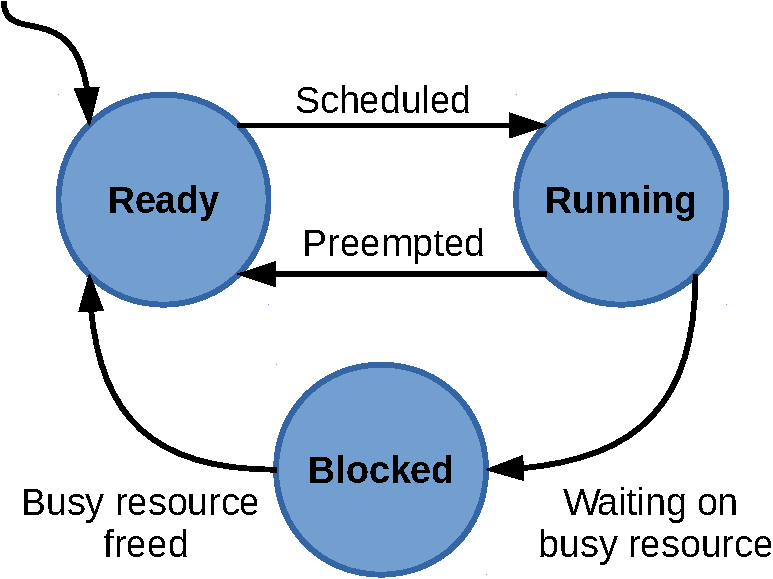
\includegraphics[width=0.7\linewidth]{images/ready-running-blocked-model.pdf}

    \caption{The three states a task may be in after its arrival and before its completion.}

    \label{fig:ready_running_blocked_model}

\end{figure}



% TOD: Introduce the notion of offline and online schedulers, start time of tasks (when they start
% execution)
% TODO: Mention Job-Level priority (JLP) and Task-Level Priority (TLP)
\section{Scheduling} \label{sec:scheduling}

Although computers give the illusion of being able to do many things simultaneously this
is actually not the case. Computers are limited to how much parallel computing they are able to do
by the hardware, specifically the amount of cores within the \acrfull{cpu}. A computer with a
single core \acrshort{cpu}, for example, is only able to execute one task at a time. In order for a
computer with a single core to deal with more than a single task at the same time it needs to switch
ongoing tasks in and out of the core during runtime. For the \acrshort{os} to switch tasks quickly
in and out of the core it needs to schedule the tasks according to some order. This is where the
priority of tasks come in handy, by scheduling tasks and switching them in and out of the processor
very quickly depending on their priority the \acrshort{os} is able to execute more than one task,
seemingly in parallel, than what is actually allowed for by the hardware. For embedded systems it is
also often of extra importance that every task is scheduled with enough time to finish before its
deadline, as not to potentially crash the system. The interval from a tasks release time until its
deadline is referred to as its \textbf{schedulability window} within which the task must be
scheduled to meet its deadline.The rest of this section up until section
\ref{subsec:multiprocessor_scheduling} is only concerned with the scheduling of single core
processors.

% TODO Maybe add other measurements of how good schedulers are, least-slack time etc.
The order in which tasks are executed is determined by the scheduler which in of itself is a special
type of task executed by the \acrshort{os}. The scheduler is invoked by specific events happening in
the system. It could for example be that a task is finished executing or that it has begun waiting
on some resource that is not yet available or a new task is released and ready to start execution.
As not all scheduling algorithms were created equal they vary in how good they manage to schedule
the same task sets. Because of this some measurements must be introduced in order to make a fair
comparison of how well they work. The processor utilization ratio, denoted as $ U $, is such a
measurement introduced to show to what percentage a specific task set would keep the processor busy.
The utilization can be calculated as $ U = \sum_{i=1}^n \frac{C_i}{T_i} $. So a very good scheduling
algorithm would be able to schedule task sets with a high utilization ratio without any of the tasks
missing their deadline. 

For embedded systems there exists a set of well known scheduling algorithms such as \acrfull{edf}
and \acrfull{rms}. Imagining a single-core \acrshort{cpu} the algorithm \acrshort{rms} works by
setting the priority of each task equal to its period. This means that the task with the lowest
period is given the highest priority and always scheduled first once it is in the ready state. Since
periods of tasks never change during execution, the priorities of the individual tasks will never
change either, thus \acrshort{rms} is said to be a \textbf{static-priority scheduler}. If a
scheduler instead changes the priorities of the task during execution, such as \acrshort{edf}, it is a
\textbf{dynamic-priority scheduler}. 

Instead of setting priorities according to the periods \acrshort{edf} works by setting the
priorities according to how close a task is to its deadline. This means that the task closest to
missing its deadline will always be executing first on the processor. If some task $ \tau_a $ is
executing with a deadline further away in time than another task $ \tau_b $, that was just released,
then $ \tau_a $ will get preempted and the newly released $ \tau_b $ will be allowed to execute
instead. This version of \acrshort{edf} is known as a \textbf{preemptive scheduling algorithm}, the
opposite of which is a \textbf{non-preemptive scheduling algorithm} which lets each task finish its
execution, even when higher priority tasks are ready to execute. The timing analysis explored in
later parts of the thesis only deals with scheduling algorithms that are non-preemptive.

An example of how \acrshort{rms} would schedule a task set can be seen in figure
\ref{fig:rate_monotonic_scheduling}. A special point of interest is at time 4 when $T_3$ is
executing while $T_1$ is released. Due to $T_1$ having a lower period than $T_3$ it also has a
higher priority. The scheduler preempts $T_3$ and lets $T_1$ execute instead. $T_3$ is later allowed
to resume execution of $T_3$ at time 5. This is what is meant by a pre-emptive scheduling algorithm.

\begin{figure}

    \centering

    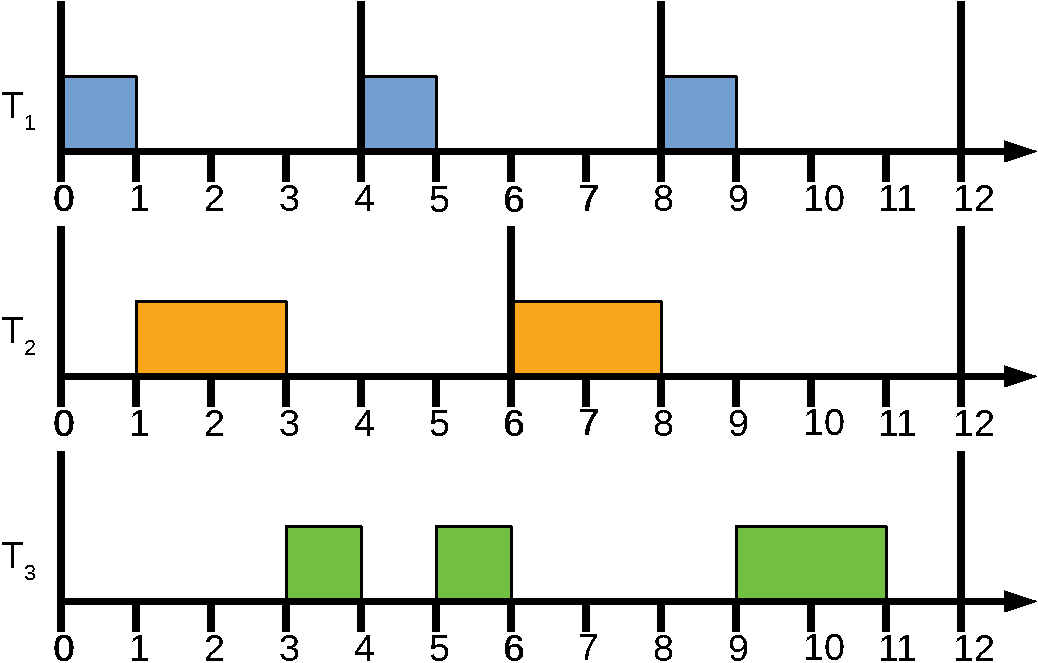
\includegraphics[width=0.8\linewidth]{images/rate-monotonic-scheduling.pdf}

    \caption{Example of rate monotonic scheduling for three tasks where $T_1=(1, 4, 4)$, $T_2=(2, 6,
    6)$, $T_3=(4, 12, 12)$. Dashed boxes represent a task waiting to resume execution after being
    preempted.} 

    \label{fig:rate_monotonic_scheduling}

\end{figure}

When considering preemptive single-core systems with static-priority assignments where the tasks
periods equal the tasks deadlines the scheduling algorithm \acrshort{rms} is guaranteed to find a
feasible schedule if such a schedule exists, making it an \textbf{optimal} scheduling algorithm
under these circumstances. For preemptive dynamic-priority assignment single-core systems
\acrshort{edf} has been proven to always find a feasible schedule if one exists, making it optimal
in those circumstances. If an algorithm however is unable to find a feasible schedule, even when
such a schedule exists, it is considered a \textbf{heuristic}.

\subsection{Multiprocessor scheduling} \label{subsec:multiprocessor_scheduling}

When considering multi-core processors life for schedulers become a little harder. On a single-core
processor the scheduler only needs to consider temporal allocation of the task, as in
\underline{when} they should run. Scheduling tasks on a multi-core system also requires the
scheduler to consider spatial allocation of the tasks, as in \underline{where} they should run
(on what core). Schedulers can deal with these allocations in two different ways, either through
what is known as \textbf{global scheduling} or through \textbf{partitioned scheduling}. 

%TODO: Mention some examples of multi-core scheduling algorithms (gEDF, RMS, etc)
%TODO: maybe have pros and cons for partitioned and global scheduling
%TODO: Maybe have a picture to help explain the differences between partitioned and global
%scheduling. This contains a good example:
%http://retis.sssup.it/~giorgio/slides/cbsd/mc3-global-2p.pdf
Partitioned scheduling entails that each task is assigned to a dedicated core which is the only core
the task is allowed to execute on, even when other cores are free. Due to this any single-core
scheduling algorithm can be used individually on each core during runtime. It is then possible to
also use the existing scheduling analysis methods for the respective scheduling algorithm. This
sounds easy enough, but in reality assigning tasks to cores is a version of the bin packing problem
which is known to be a NP-hard problem meaning that there exists no algorithm to solve it in less
than polynomial time. However, good heuristics
\parencite{johnson_fast_1974}\parencite{coffman_application_1978} exists that find good solutions
fast and since tasks can be allocated to cores offline more computing power and time can be used to
find close to optimal solutions than if it had to be done during runtime.

Global scheduling means that the scheduler takes into account both spatial and temporal allocation
when scheduling each task. Algorithms from sing-core scheduling can be applied to global scheduling
such as \acrshort{rms} and \acrshort{edf}, but they will have different behaviour. Global scheduling
decreases the determinism of the system and creates more combinations of possible schedules for each
task set. This makes global scheduling much harder to run analysis on.

All of the algorithms explored this far have taken a \textbf{core-centric} approach to scheduling tasks,
meaning they see the cores as the resources and try to assign tasks to them as efficiently as
possible. Another possibility is to take a \textbf{memory-centric} approach to scheduling instead.
As the amount of cores in a processor increases so does the usage of shared memory to a point where
increasing the cores further will not increase the schedulability ratio as the shared memory
bottlenecks the system by being busy non-stop. Memory accesses can then be scheduled explicitly such
that tasks have assigned time slots within which they are allowed to access the shared memory. Since
there usually is only one shared memory this also reduced the problems of multi-processor scheduling
down to  single-processor scheduling as there is a single resource to for the tasks to be scheduled
on. How a memory-centric approach can be implemented is discussed in the rest of the thesis.

\section{Schedulability analysis} \label{sec:schedulability_analysis}

%TODO mention brute-forcing analysis by simulating one hyper period of the schedule. And this seems
%easy in theory, but in practice there can be hundreds of tasks and super long hyper period.
When developing new scheduling methods it is important to put the schedules that they produce under
analysis as to show whether they are feasible or not. It is especially important when the schedules
are used in hard real-time systems like those found in the avionics and the automotive sector where
missed deadlines could mean fatal outcome. For example, \acrshort{rms} can be analysed
mathematically and has been proven to be able to schedule any task set that fulfills the constraint
$ U \le n(2^{\frac{1}{n}}-1) $ where $ n $ is the amount of tasks \parencite{liu_scheduling_1973}.
This is only a \textbf{sufficient} condition, meaning that \acrshort{rms} might be able to schedule
task sets that do not fulfill the condition, but it is not guaranteed to. On the contrary, a
condition that must be fulfilled for the task set to have a feasible schedule, but does not
guarantee such a schedule exists, is known as a \textbf{necessary} condition. If a condition is both
necessary and sufficient it is said to be \textbf{exact} which means that if the analysis deems a
task set to be schedulable it is guaranteed to be schedulable, and if it deems it not to be
schedulable it is guaranteed not to be schedulable. An example of an exact condition for
\acrshort{edf} on single-core processors is $ U(\Gamma) \leq 1 $ which states that the utilization
of the task set must be one or less. Finding good conditions is not always trivial as shown by
\parencite{bini_hyperbolic_2001} which presents a less pessimistic sufficient condition for
\acrshort{rms} of the same complexity $ O(n) $ almost 30 years after the first presented condition
was introduced. 

%TODO: Mention that increase of tasks leads to harder schedulability
%TODO: Mention that the illustration is mostly to get and idea of the problem trying to be solved,
%and that it represents single-core and a multi-core representation would look slightly different
%(due to a single task not being able to utilize all cores), but the idea is the same.
The gap between sufficient conditions and necessary conditions where the tasks sets are undetermined
if they are able to be scheduled is illustrated in figure
\ref{fig:sufficient_necessary_schedulability}. A lot of research is being aimed towards finding less
pessimistic necessary and sufficient conditions for scheduling algorithms to close the gap between
them which is still not a solved problem in all cases. In addition, each unique scheduling algorithm
may require its own set of unique conditions for analysis. All conditions are also not as simple as
the one presented for \acrshort{rms} especially when also considering multi-core. The conditions
have varying complexity and they often need to make the trade-off between complexity and how
pessimistic they are. The paper \parencite{bertogna_tests_2011} shows examples of conditions that
are of $ O(n^3) $ complexity which can be alright when analysing small task sets, but is too complex
as the task sets grow or if it has to be calculated during runtime with limited computation power.

\begin{figure}

    \centering

    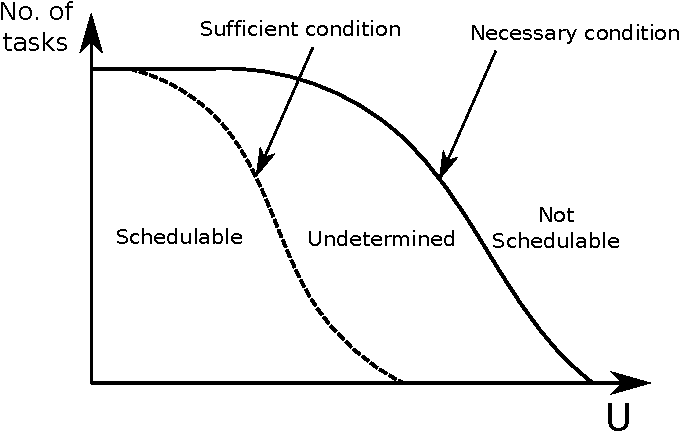
\includegraphics[width=0.8\linewidth]{images/sufficient_necessary_schedulability.pdf}

    \caption{Research aims to shrink the gap left between sufficient and necessary conditions.
    Illustration inspired by \parencite{sebestyen_simulation-based_2012}.}

    \label{fig:sufficient_necessary_schedulability}

\end{figure}

% TODO: Is this section really necessary? Perhaps preface with it by explaining there are different
% ways of analysis. Other than mathematically, we can also simulate the schedule and look for missed
% deadlines. Don't use the word simulation, we are only doing analysis, otherwise people will be MAD
% TODO: Critical instant is worst case for a specific task. Only for RMS and EDF is this when all higher
% prio tasks are released at the same time.
An example of a precise schedulability test for \acrshort{rms} on single-core systems is to find the
so called \textbf{critical instant} of a task. This is when all higher priority tasks are released
at the same time as the task. This pushes the task completion time as far away from its release time
as it ever will be in the given task set. If the task doesn't miss its deadline after the critical
instant it is guaranteed to never miss its deadline for any other instance in the schedule. As an
effect of this, each task can be examined during its critical instant, and if all tasks meet their
deadlines the task set is guaranteed to be schedulable. This simplifies analysis considerably as
only a small part of the schedule needs to be analysed.

However, having the arrival and computation time defined as intervals creates the possibility of
different schedules for the same task set using the same scheduler. This makes analysis more
difficult as analysis requires testing several of the combinations of release and computation times.
It is intuitive to think that it is sufficient to analyse the worst-case times of all tasks to find
if the schedule is feasible. This is however not true for non-preemptive systems as two jobs with
the same arrival-time interval can lead to either being scheduled before the other until its
completion. For some task sets with this property a later or earlier release of a certain job may
lead to a missed deadline later in the schedule. This also means that examining the critical instant
of a task is no longer sufficient in determining if a task set is schedulable or not. An example of
this phenomena can be seen in fig \ref{fig:np-test_schedule} and is further explored in the next
section.
% TODO Example of how earlier release of a task on multicore systems can make the schedule miss a
% deadline while a later release of the same task may have been able to complete the deadline.


\section{Non-Preemptive schedulability test} \label{sec:np-test}

The work which this thesis builds upon is presented in \parencite{nasri_exact_2017}. An open-source
implementation written in c++ by one of the authors is available on
Github\parencite{brandenburg_implementation_2018} and will further be referred to as the
\acrfull{np}-test. It presents an \textbf{exact} non-preemptive schedulability test for single-core
processors. The basic idea is to build a schedule graph, using vertices and edges, that fully
represents all possible schedules for a given job set input. A job set contains all the individual
schedulable instances of each periodic task in a task set and all tasks can easily be converted into
their corresponding jobs. This analysis isn't a new idea but it brings a novel merge phase that
merges all nodes of the graph that will lead to the same outcome in the future making it scale better
both in size and time. It is also able to take into account uncertainties in the job set to better
reflect reality by taking both release-time jitter and the \acrshort{bcet} and \acrshort{wcet} into
consideration. The test is both sufficient, necessary and sustainable. Where sustainable is defined
as "A schedulability test is defined to be sustainable if any task system deemed schedulable by the
test remains so if it behaves 'better' than mandated by its system
specifications"\parencite{baruah_sustainable_2006}. Thus also making it exact.

The analysis tool is also able to deal with non-work-conserving schedulers by accepting an
\acrfull{iip} function. An \acrfull{iip} is used during scheduling to see if the highest priority
task is to be scheduled at the present time when there is a free core to schedule the task onto or
if the core should be left idle. The idea is that a non-work-conserving algorithm can increase
schedulability by trying to make smarter scheduling choices such as delaying a low priority job if a
high priority job is expected to be released in the near future. Two existing \acrshort{iip}'s are
already implemented in the \acrshort{np}-test, the first one is \acrfull{p-rm}
\parencite{nasri_precautious-rm:_2014} and the second \acrfull{cw-edf}
\parencite{nasri_non-work-conserving_2016}.

A job-set containing 9 unique jobs derived from the tasks $\tau_1=([3,13], 60, 60)$, $\tau_2=([7,
8], 30, 30)$ and $\tau_3=([1,2], 10, 10)$, no release jitter is assumed, is presented in
\parencite{nasri_exact_2017}. These are scheduled according to figure \ref{fig:np-test_schedule}
when every job executes for its \acrshort{wcet} and the result is that they all meet their
deadlines. However, if $J_7$ would instead execute for one time unit \textbf{less} it would result in the
schedule depicted in figure \ref{fig:np-test_schedule_fail} where $J_2$ misses its deadline. This
example perfectly shows the problem with analysing non-preemptive scheduling as it is not sufficient
to just check if all deadlines are met when all jobs execute for their \acrshort{wcet}. The task-set
is shown to become feasible if the priorities are reordered as $ p_1 < p_2 < p_3 < p_4 < p_5 < p_5 <
p_9 < p_7 < p_8$.


\begin{figure}

    \centering

    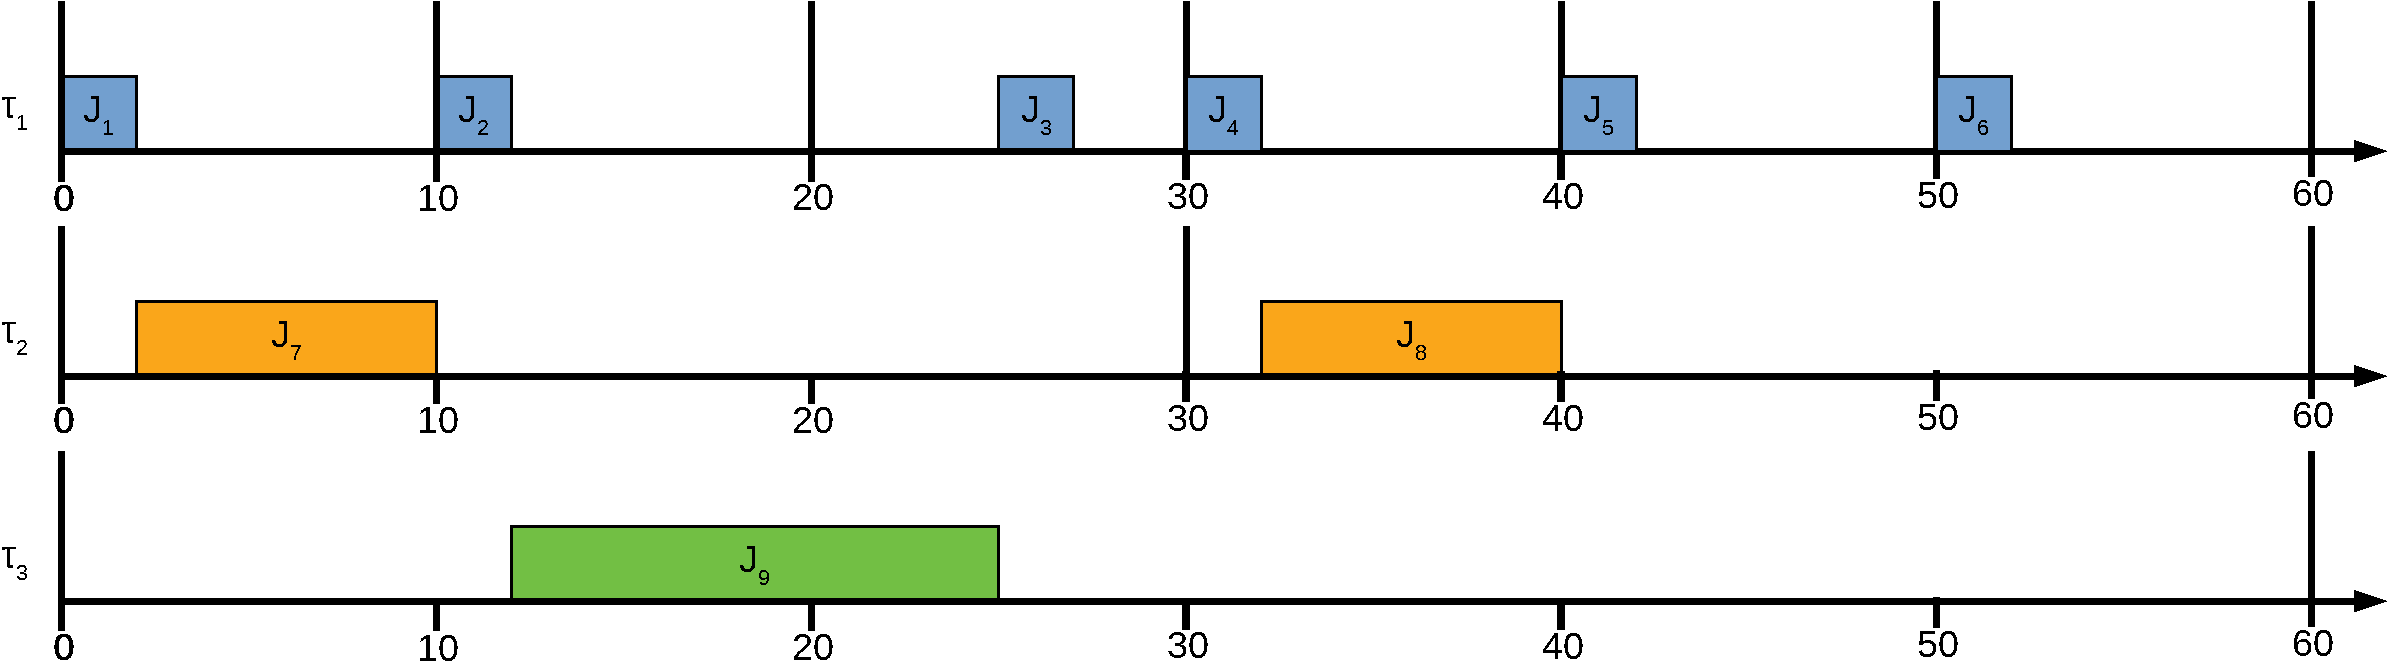
\includegraphics[width=1.0\linewidth]{images/np-test_schedule.pdf}

    \caption{Non-preemptive task-set scheduled under \acrshort{edf} or \acrshort{rms}}

    \label{fig:np-test_schedule}

\end{figure}


\begin{figure}

    \centering

    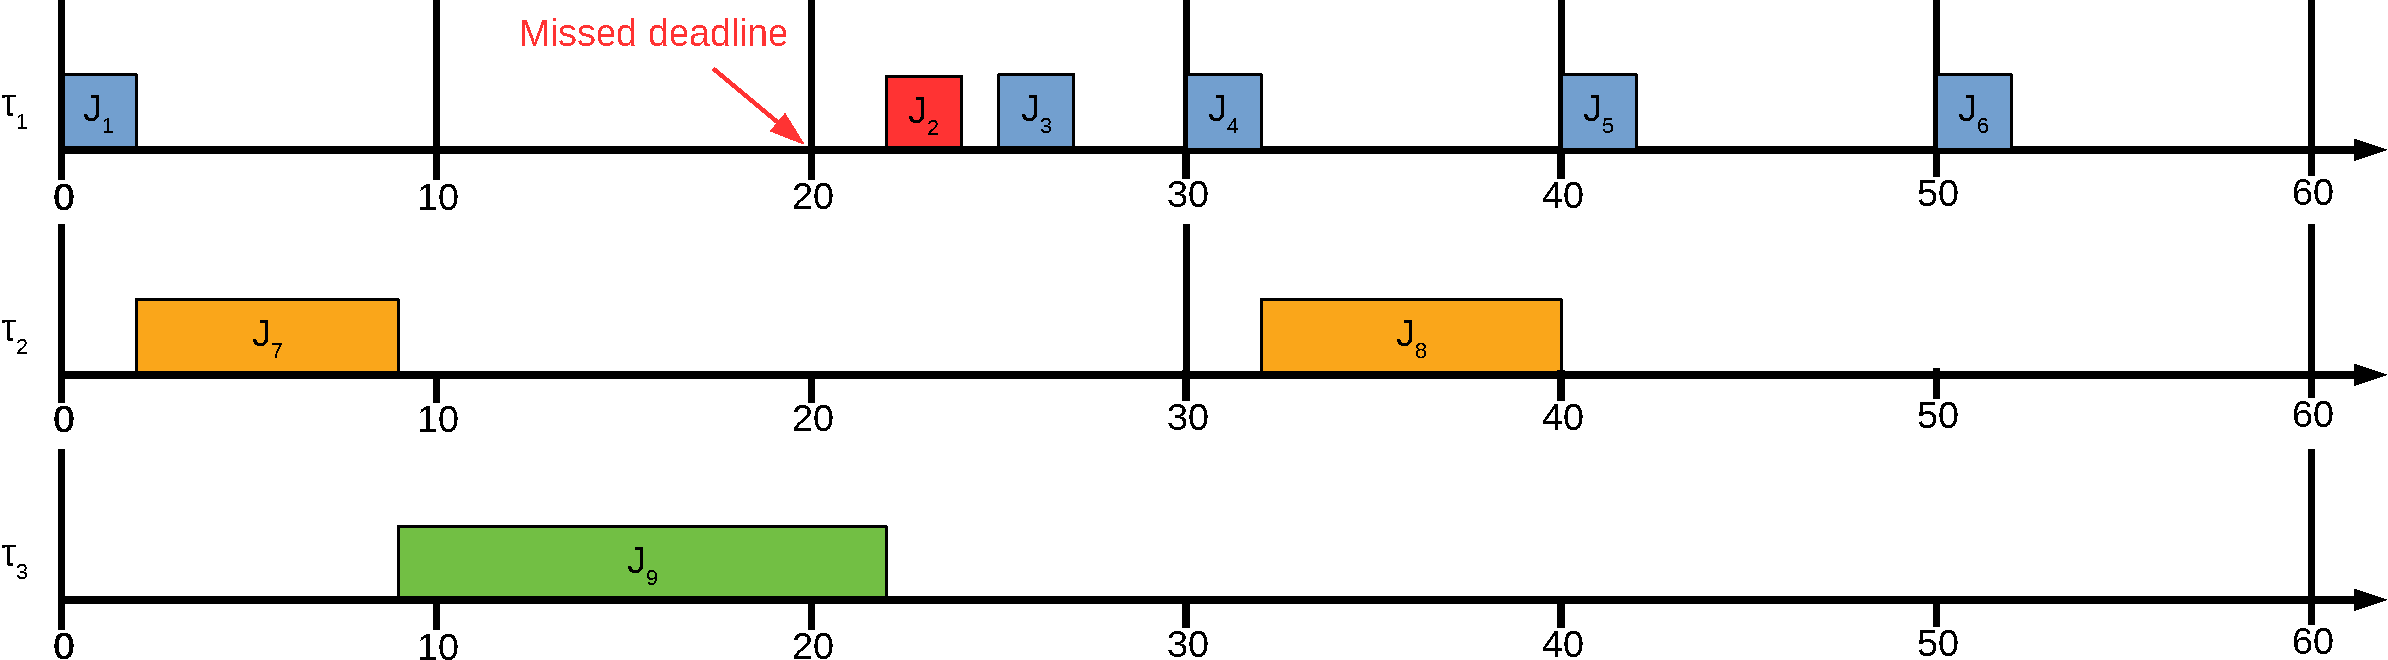
\includegraphics[width=1.0\linewidth]{images/np-test_schedule_fail.pdf}

    \caption{Non-preemptive task-set where $J_7$ finishes 1 time unit earlier, scheduled under
    \acrshort{edf} or \acrshort{rms}}

    \label{fig:np-test_schedule_fail}

\end{figure}


The scheduling graph is a \acrfull{dag} where each edge represents a scheduling decision and each
node represents a time-interval. The graph is built from the root node by making scheduling
decisions. Looking back at the job-set from the previous paragraph, part of its scheduling graph
would be represented by the \acrshort{dag} depicted in figure \ref{fig:scheduling_graph} when
scheduled under \acrshort{edf}. From the root node $v_1$ the highest-priority job of all available
jobs is scheduled, job $J_1$, and an edge is added to represent it. The other end of the edge is
connected to a new node $v_2$ that represents the interval within which the scheduled jobs may
finish execution. Since the \acrshort{wcet} is 2 and \acrshort{bcet} is 1 for $J_1$ the interval for
the new node is $[1, 2]$. For all points in time within this interval the highest priority-job that
has been released is job $J_7$ and is thus scheduled. Its \acrshort{wcet} is 8 and its
\acrshort{bcet} is 7.  These are added to the interval of the possible finish times from the
previous node and creates the new interval $[8,10]$. Now there are two scheduling possibilities that
are dependent on when the previous jobs have finished execution. If $J_7$ finishes before time 10
then $J_9$ will be the highest priority released job, and if $J_7$ finishes at time 10 then $J_2$ is
the highest priority released job. Since two different scheduling decisions can be made within the
interval represented by node $v_3$ two new edges are branched out from that node, each representing
one of the two scheduling decisions. If $J_2$ is scheduled it must start at time 10, to this is
added its \acrshort{wcet} 2 and \acrshort{bcet} 1 to create the interval represented by the node
$v_5$. If $J_9$ is scheduled it can start within the interval $[8, 9]$, and thus its \acrshort{wcet}
13 and \acrshort{bcet} 3 is added to that interval to create node $v_4$. At this point each of the
two branches continue scheduling jobs and branch out whenever several options are available until
either all jobs have been scheduled, or a job fails to meet its deadline. This will for large job
sets create a huge search space that is very computation and memory intensive and does not scale
very well. However, the novelty of the approach presented in \parencite{nasri_exact_2017} is to
introduce a merge-phase. The merge phase tries to decrease the search space by merging vertices that
lead to similar execution scenarios. The criteria for merging two vertices is that (a) the same jobs
have been scheduled before the vertices and (b) the finish-time interval they both represent
overlaps, i.e. $v_i \cap v_j \neq \emptyset$.  When this is the case the new vertex $v_n$ that is
created from the merge represents the union of finish times from the two merged vertices $v_i$ and
$v_j$ as such $v_n \gets v_i \cup v_j$. Both of these criteria are fulfilled for vertices $v_4$ and
$v_5$ meaning that they can be merged into a single vertex. The merging is illustrated in figure
\ref{fig:scheduling_graph_merge} which also shows the edges that no longer needs to be explored
using dashed lines.

\begin{figure}

    \centering

    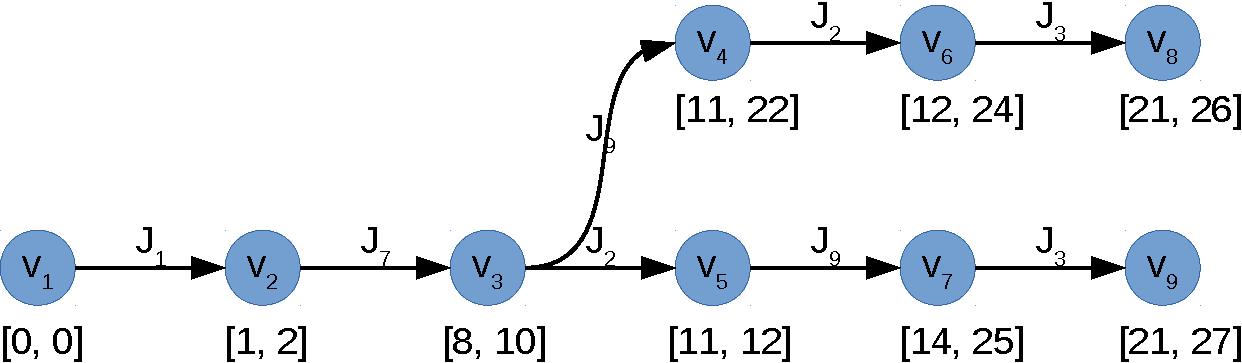
\includegraphics[width=0.8\linewidth]{images/scheduling_graph.pdf}

    \caption{Example of the \acrshort{dag} scheduling graph with a branch representing two different
        scheduling possibilities.}

    \label{fig:scheduling_graph}

\end{figure}


\begin{figure}

    \centering

    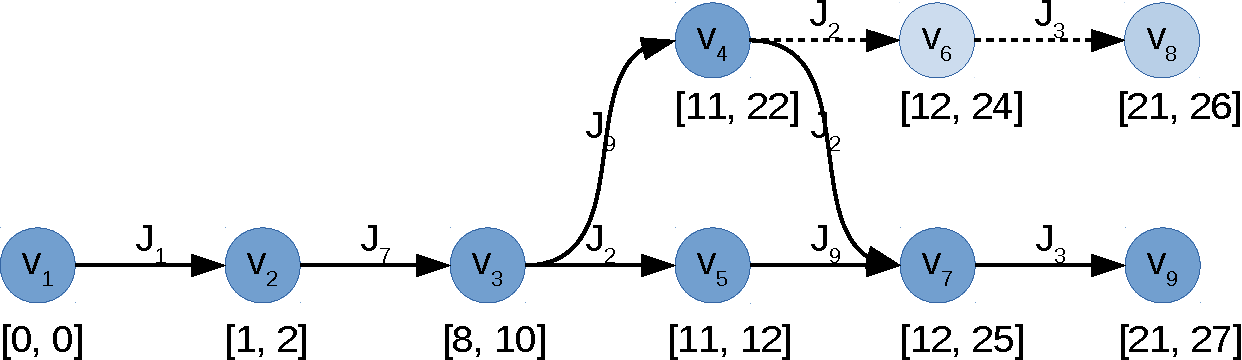
\includegraphics[width=0.8\linewidth]{images/scheduling_graph_merge.pdf}

    \caption{Example of the \acrshort{dag} scheduling graph merging two nodes that lead to the same
    outcome.}

    \label{fig:scheduling_graph_merge}

\end{figure}

\section{The AER Execution Model} \label{sec:aer_execution_model}

The \acrfull{aer} execution model was first presented in \parencite{durrieu_predictable_2014} to
improve performance and predictability while using \acrfull{cots} multi-core processors with shared
and private memory in the avionics industry. It builds on top of the \acrfull{prem} first presented
in \parencite{pellizzoni_predictable_2011} which introduces the idea of dividing tasks into a memory
access phase and an execute phase. Since the bottleneck for utilization in multi-core systems can
become the contention in access to shared memory when introducing an increasing number of cores
\acrshort{aer} focuses on making shared memory access more deterministic and easier to analyse. This
is done by dividing up each task into three distinct parts. The \textbf{acquisition} (A) part reads all
the data necessary for execution of the task such as code and shared variables into the private
memory of the core dedicated for execution. The \textbf{execution} (E) phase then executes the code
operating on local copies of any shared variables without making any further read or write
instructions to the shared memory. The \textbf{restitution} (R) phase then writes back all of the
acquired results that may be needed of the task to the shared memory. Since the \acrshort{a}-phase
only is allowed to execute before execution of the task actually starts a pre-requisite of the model
is that each core has a separate private memory, such as a cache or a scratchpad. Since these types
of memories often are constrained in size it puts a limit to how many instructions a task can
consist of in addition with the amount of shared variables that is used as they all must fit in
the private memory of the core.

The idea of this model is to enable scheduling of the read and write accesses to the shared memory
instead of scheduling the tasks onto cores. Since contention of the shared memory may be what limits
the utilization of the cores it is more important to combat this instead of trying to find the
optimal assignment of tasks onto cores since it wont increase utilization anyways. \acrshort{aer}
can be said to employ a \textit{memory-centric} approach to scheduling instead of a
\textit{core-centric} approach that schedulers usually employ. This model also has the advantage of
easier analysis by being more deterministic. When several cores compete for resources and create
congestion which leads to timing deviations the system model becomes more complex thus harder to
analyse. Timing that was calculated offline, for example the \acrshort{wcet}, may not match reality
or require very pessimistic approximations that exaggerate the timings, both of which decreases the
certainty or predictability of the design and analysis.

There exists some scheduling algorithms and timing analysis tools developed for the \acrshort{aer}
model such as the one proposed in \parencite{durrieu_predictable_2014} that is a partitioned
non-preemptive offline scheduler. The paper \parencite{maia_closer_2016} further evaluates the
\acrshort{aer} model by testing different scheduling algorithms. Instead of using offline partial
scheduling it proposes five different heuristic algorithms under online global scheduling. These
algorithms assign a higher task priority according to period (\acrshort{rms}), shortest acquisition
phase, longest acquisition phase, shortest restitution time and longest restitution time. It is
shown through analysis that the \acrshort{rms} scheduler is far best in terms of schedulable task
sets as their utilization increases. The paper \parencite{becker_contention-free_2016} explores
further ways of scheduling under an \acrshort{aer} model by proposing a global scheduling algorithm
that is shown to only behave 0.5\% worse than an optimal \acrfull{ilp} algorithm in a fraction of
the time.

% AER is an improvement over other models such as proposed by pikeOS which enables all other cores
% to be paused while running critical tasks on a single core.


\section{Related Work} \label{sec:related_work}

The most important paper is \parencite{nasri_exact_2017} which provides a state-of-the-art
schedulability analysis method for non-preemptive static-priority task sets for single-processors.
The analysis is exact for single-core systems and a corresponding sufficient analysis method for
multi-core systems by the same authors is presented in \parencite{nasri_response-time_2018}. The
concept behind the single-core analysis is explained fully in section \ref{sec:np-test}. Since the
multi-processor analysis method build on the same concepts as the analysis for single-processors it
is also of interest and is summarized in section \ref{subsec:artafnpjsug}. Since the thesis also
builds on top of the concept of the \acrshort{aer} model it is necessary to be familiar with the
paper \parencite{durrieu_predictable_2014} which was the first to present this model and presents an
offline non-preemptive partitioned scheduling algorithm to schedule the memory accesses. This paper
and the \acrshort{aer} model is explained in detail in section \ref{sec:aer_execution_model}.

The idea to divide up tasks into distinct execution phases is not a novel one as \acrshort{aer}
builds on top of the \acrshort{prem} which divides up tasks into a read and execute phase for
single-core system and was first presented in \parencite{pellizzoni_predictable_2011}. The
\acrshort{aer} model is also further explored in \parencite{maia_closer_2016} which presents five
new global non-preemptive online scheduling algorithms where the most successful assigns priorities
to tasks based on their period in the same way \acrshort{rms} works. It is also shown to be able to
schedule tasks sets that would otherwise not be schedulable under global \acrshort{edf} due to
congestion.

%TODO: Mention that this does no take into the account the deadline of the R-phase.
%TODO: Maybe keep all related work covering scheduling analysis in a new subsection
Some work on analysing have been done on analysing the schedulability of algorithms developed around
\acrshort{prem} such as \parencite{alhammad_schedulability_2014} which builds on the idea of a
problem window from \parencite{baker_multiprocessor_2003}. The paper presents an analysis method for
\acrshort{edf} and \acrfull{dms} on multi-core processors and defines the problem window as the
time interval between the release time and deadline of a certain task $ \tau_i $. The method works
by contradiction where the task is assumed to miss its deadline within the window. An upper bound $
UB(\psi_i) $ of the interference in the timing window $ \psi_i $ is defined as the maximum amount of
utilization that the task set $ \Gamma $ could possibly generate inside the timing window. The lower
bound $ LB(\psi_i) $ is then defined as the demand required on the problem window for $ \tau_i $ to
miss its deadline. The condition $ UB(\psi_i) \le LB(\psi_i) $ then defines a sufficient
schedulability condition for work-conserving schedulers if it is shown to hold for every task in the
task set. The paper also extends the \acrshort{prem} to a multi-core scheduler and called
\acrshort{gprem} which is a global static-priority scheduler. This scheduler is shown to, on
average, schedule more task sets than a baseline global round robin scheduler that does not account
for contention. The different cases tested for were different utilization, different period ranges,
different tasks per core and different number of cores for the scheduling algorithms.

The paper \parencite{maia_schedulability_2017} specifically tackles analysis for the \acrshort{aer}
model for multi-core systems by using the theory of problem windows but applying it in a bus-centric
way. The idea is that by doing analysis of the scheduling of bus accesses instead of the cores it
becomes a single-core problem as only one core can access the bus at a time.  Instead of checking
for an upper bound of the interference that tasks create on cores the method describes a way to find
the upper bound of the interference on the bus created by the other tasks. A bus hole is defined as
"\textit{A bus hole is an interval of time, within the problem window, where all m cores are busy
executing E-phases}" \parencite{maia_schedulability_2017}. The amount of time within all the bus
holes inside the problem window must be enough for the task being examined to schedule its A and R
phases to be able to meet its deadline. The paper describes a method that can compute an upper bound
on the holes in the problem window in pseudo-polynomial time.

The paper \parencite{becker_contention-free_2016} makes an effort to adapt the \acrshort{aer} model
to real applications in the automotive domain by providing a general framework that is applied to
the physical platform Kalray MPPA-256. It consists of 16 compute clusters that contain 16 processing
elements and 16 banks of shared parallel memory each. The concept builds on top of the
\acrshort{autosar} architecture for automotive \acrshort{ecu}'s where the smallest unit of execution
is known as a runnable. Runnables communicate with each other through variables called labels. For
each compute cluster one memory bank is reserved as the shared memory which stores all of the
labels, thus referred to as the label bank. The remaining 15 memory bank are then each assigned as a
private memory to a unique processing element. The runnables running on the processing units are
then executing under the \acrshort{aer} model. A scheduler is then presented to schedule the memory
access phases of the runnables to battle congestion. The scheduling algorithm is said to be a
\textit{memory-centric heuristic} as it schedules the A and R phases on the memory as opposed to a
\textit{core-centric heuristic} that schedules tasks onto cores.

% - autosar, labels, runnables
% - physical hardware platform (MANY-core)
% - scheduler

\subsection{A Response-Time Analysis for Non-Preemptive Job Sets under Global
Scheduling}\label{subsec:artafnpjsug}

%TODO: Mention it requires static-priority assignment
The paper \parencite{nasri_response-time_2018} presents a state-of-the art analysis method for
non-preemptive multi-processor global scheduling. The method gives a sufficient condition for
schedulability. The input is a set of jobs consisting of their ID, deadline, priority, earliest
release time, latest release time, \acrshort{wcet} and \acrshort{bcet}. The output then tells
whether or not the input is schedulable. The basic idea of the analysis is to enumerate all of
possible combinations of \acrshort{wcet}, \acrshort{bcet} and release jitter but as not to be
computation- or memory-heavy it tries to be clever about it. This is done by removing all duplicates
of schedules that lead to the same ordering of start times for the jobs.

The implementation of the analysis works much like its single-core version by progressively building
a tree graph where each edge represents a scheduling decision in the form of a specific job assigned
to a specific core. The root node represents the start of scheduling when the first job is
available, usually at time zero. If two jobs are able to be scheduled during the same interval they
will be represented as two different edges in the graph stemming from the same node. Each node
represents a state in time of the schedule and contains information about the interval between the
earliest possible availability and latest possible availability of each core (the time at which a
core is ready to accept a new job) in the system. The root node represents time zero in the schedule
at which no job yet has been assigned to any core. 

The tree graph is built progressively by iterating the algorithm through three different phases.
The expansion phase selects the shortest path (as in the amount of edges)from the root to a leaf
node and makes a scheduling decisions (assignment of ready job onto vacant core) at the leaf node
and creates the corresponding edge. A unique edge is created for each core that the job may be
assigned to. Each assignment leads to a certain state of the schedule represented by an added leaf
node. The fast-forward phase then progresses time until the next scheduling decision is to be made
(a core has become vacant). The final phase, the merge phase is the part where the analysis is
clever by trying to minimize the search space of the tree graph. Paths that have scheduled the same
job sets in different order but have the same timing values will lead to identical sub-trees in the
future. Because of this it is only necessary to continue evaluation from one of the nodes
effectively making it so that the nodes can be \textit{merged} by following certain rules.


\chapter{Method} \label{ch:method}

This chapter explains the work that has been done to reach the conclusions in the thesis. Section
\ref{sec:work_task_model} presents an extended version of the \acrshort{aer} task model that has
been developed. Section \ref{sec:iip} presents a new \acrshort{iip} that can be used in conjunction
with the \acrshort{np}-test in order for the test to accept job-sets of the \acrshort{aer} task
model presented in section \ref{sec:work_task_model}. Section \ref{sec:scheduling_algorithms}
presents the scheduling algorithms that will be used during benchmarking to prioritize the jobs.
Section \ref{sec:benchmarking} discusses how benchmarking was done to get correct results to
evaluate the task model presented in section \ref{sec:work_task_model} and the different scheduling
algorithms presented in section \ref{sec:scheduling_algorithms}.

\section{Task model} \label{sec:work_task_model}

When the interval between the worst-case finish time of the \acrshort{a}-phase and the best-case
release time of the \acrshort{r}-phase is less than the \acrshort{wcet} of the \acrshort{e}-phase a
problem arises. The \acrshort{np}-test timing analysis can't make the guarantee that the interval
between the finish time of the \acrshort{a}-phase and the start time of the \acrshort{r}-phase is
sufficient for the \acrshort{e}-phase to finish its execution. The problem becomes even worse as the
schedulability windows of the \acrshort{a}-phase and \acrshort{r}-phase overlaps as the analysis
doesn't handle any precedence constraints among jobs. This means that it would be possible for an
\acrshort{r}-phase to be scheduled before the \acrshort{a}-phase belonging to the same job.

As explained, it is a property of the model that an \acrshort{a}-phase must always precede its
matching \acrshort{r}-phase belonging to the same task. It also becomes more complicated than a
simple precedence constraint as the analysis must leave sufficient time between the finish time of
the A-phase and the start time of the R-phase for the E-phase to finish execution. This can be
circumvented by introducing new concepts to the \acrshort{aer}-model. The schedulability window of a
task can be divided into three non-overlapping intervals that can be thought of as sub-windows of
the schedulability window. The first window is referred to as the acquisition-window and is the
interval within which the \acrshort{a}-phase is allowed to execute within. The second interval
begins right after the first and is the size of the \acrshort{wcet} of the \acrshort{e}-phase as it
is the required time before the \acrshort{r}-phase is allowed to start execution. After the second
interval is the \acrshort{r}-window within which the \acrshort{r}-phase is allowed to execute. So
each phase has a predetermined interval as a part of the whole schedulability-window where no
intervals are allowed to overlap. This concepts is illustrated in figure \ref{fig:aer_window_model}.


\begin{figure}

    \centering

    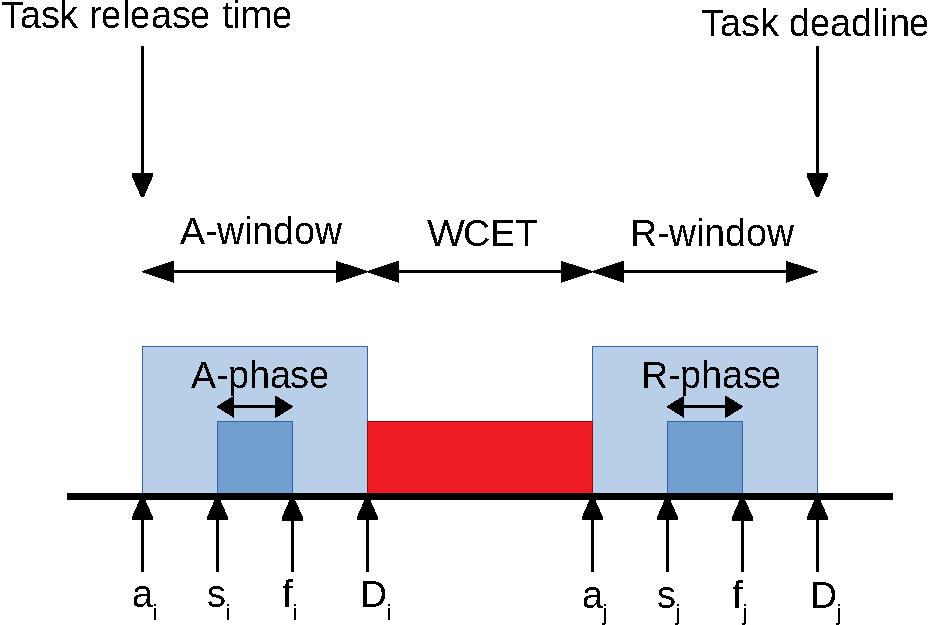
\includegraphics[width=0.8\linewidth]{images/aer_window_model.pdf}

    \caption{The AER window model, note that the \acrshort{a}-phase and \acrshort{r}-phase can be
    scheduled during any time within their windows.}

    \label{fig:aer_window_model}

\end{figure}


The task within each of its period is in this way divided into two separate jobs, the first job,
denoted $ J^{A} $, represents the \acrshort{a}-phase and the second job, denoted $ J^{R} $, representing
the \acrshort{r}-phase. Each of the jobs arrival time and deadline are then set to correspond to its
scheduling window as seen in figure \ref{fig:aer_window_model}. Each individual job then represents
accesses to the shared memory and can be scheduled by a regular scheduler as if they were regular
jobs being scheduled on a single core, which is why the multi-core problem is in a way reduced to a
single-core problem when developing memory-centric heuristics. In this way the \acrshort{r}-phase
doesn't have to worry about if the \acrshort{a}-phase and the \acrshort{e}-phase have yet to finish
execution as a property of the model is that the restitution-phase will never be released before the
execution-phase is guaranteed to have finished even in the worst-case. One interesting property of the
model is that the interval for the \acrshort{a}-phase and \acrshort{r}-phase doesn't necessarily
have to be of the same size, but more time could for example be allocated for the
\acrshort{a}-window with a cost of shrinking the \acrshort{r}-window. The relationship between the
size of the two intervals is referred to as the \textbf{window-ratio} and is equal to the size of
the \acrshort{a}-windows size divided by the sum of the \acrshort{a}-windows and
\acrshort{r}-windows sizes. This is explored further during benchmarking in section
\ref{sec:benchmarking}.

It quickly becomes obvious however that the model has some disadvantages. The most obvious one being
that the core which the task is assigned to might idle for a long time during certain circumstances.
For instance, even though enough space is allocated between the \acrshort{a}-window and
\acrshort{r}-window for the \acrshort{e}-phase to finish there is nothing prohibiting the
\acrshort{e}-phase from starting execution as soon as the \acrshort{a}-phase is complete, even if
this is well before its deadline. So when the \acrshort{a}-phase and \acrshort{e}-phase finish
executing, especially in the best case, the restitution phase is yet to be released for what may be
a very long time, thus leaving the allocated core idle for all of this time while unable to finish
its \acrshort{r}-phase even though it should be able to. Another problem is that the number of tasks
with the same period can never be larger than the amount of physical cores as such a task set never
can be schedulable. This is illustrated by imagining a task set where all tasks have the same
periods and same window-ratio. All but on task is then being assigned cores at the same time such
that all cores are busy. The occupied cores would then be busy until the restitution-phases are
finished executing, at which time the acquisition-phases are all guaranteed to have had their
deadlines passed, thus the unassigned task will miss its deadline. The effect of these disadvantages
are further discussed in chapter \ref{ch:results}.


\section{Idle-time Insertion Policy} \label{sec:iip}

% TODO: Explain IIP in theoretical framework instead?
% TODO: Mention IIP-eligibility

% TODO: Move to background "work-conserving vs. non-work-conserving"
Imagining a non-preemptive scheduler and a long-running, low-priority task with a deadline far into
the future that has just been released and is about to be scheduled onto a single-core system. If a
higher-priority task with a short deadline is then released just after the first task has been
scheduled the second task might miss its deadline as the core wont be available for a long time. In
this instance it could prove beneficial for scheduling algorithm to leave a core idle even when
there is work to be completed to wait for a higher priority task to be released. This idea of
leaving core idles and postponing work is the philosophy behind using an \acrfull{iip}. An
\acrshort{iip} makes a decision about whether or not the highest priority job is to be scheduled
when the core becomes free or if the core should be idle until another higher priority job is
released.

For a basic \acrshort{iip} to make a decision about whether or not to schedule a job it is provided
with three pieces of information. First the job-set of jobs that have previously been scheduled and
are finished, second it is provided the job that just has been released and is to be scheduled,
thirdly it is provided the present time at which the released job is to be scheduled. The policy
then returns a true or false value representing if the provided job is schedulable at that time. The
usage of an \acrshort{iip} by a scheduler to check for eligibility can thus be described by
algorithm \ref{algo:iip_eligibility}, inspired by \parencite{nasri_exact_2017}.

\begin{algorithm}
    \caption{IIP eligibility}
    \label{algo:iip_eligibility}
    \begin{algorithmic}[1]
        \State $J_i\gets Highest\ priority\ released\ job$
        \State $t\gets Present\ time\ in\ the\ schedule$
        \State $\mathcal{J}\gets Already\ scheduled\ jobs$
        \State $c\gets Total\ cores\ in\ system$
        \If {$aer\_iip(J_i, t, \mathcal{J}, c) = true$}
        \Comment{Algorithm \ref{algo:aer_iip}}
            \State $schedule(J_i)$
        \Else
            \State $idle\_processor()$
        \EndIf
    \end{algorithmic}
\end{algorithm}

A problem with using the extended \acrshort{aer} model proposed in section
\ref{sec:work_task_model} with the timing analysis \acrshort{np}-test is that the analysis doesn't
know if a processing core is free when scheduling a \acrshort{a}-job as it only is concerned about
whether or not the memory is free. The \acrshort{np}-test can however be used in conjunction with
different \acrshort{iip}'s. To make sure the task model described in section
\ref{sec:work_task_model} works with the \acrshort{np}-test a custom \acrshort{aer} \acrshort{iip}
is created as scheduling tasks using a memory-centric approach in some ways is similar to a
non-work-conserving scheduler as the memory might be left idle, even when there is work to be done.

The \acrshort{aer} \acrshort{iip} needs to make sure of two things when a job is ready to be
scheduled. The first thing is to check if the job to be scheduled is an \acrshort{r}-job or an
\acrshort{a}-job. And secondly if it is an \acrshort{a}-job there has to be a check if there is an
free core for the job to be scheduled onto. This is only true for \acrshort{a}-jobs as
\acrshort{r}-jobs had their core dedicated to them when their respective \acrshort{a}-job was
scheduled. To find if there are any free cores an additional argument needs to be passed into the
\acrshort{aer} \acrshort{iip}, which is the total amount of cores in the system (whether
or not they are free). To find out the amount of free cores in the system an additional algorithm is
called from within the \acrshort{iip} with two arguments, the total amount of cores in the system
and the job-set of jobs that have been scheduled. 

In order to recognize if a job is an \acrshort{a}-job or \acrshort{r}-job without extending the
input to the \acrshort{np}-test this information can be encrypted in the jobs ID in a way where all
\acrshort{a}-jobs have an odd ID and all \acrshort{r}-jobs have an even ID. The amount of cores that
are currently occupied can then be calculated by subtracting the amount of \acrshort{r}-jobs that
have been scheduled since the beginning from the amount of \acrshort{a}-jobs that have been
scheduled since the beginning using the job set of scheduled jobs. This is explained by algorithm
\ref{algo:available_cores}. After the amount of available cores have been found as well as if the
job to be scheduled is an \acrshort{a}-job or \acrshort{r}-job a decision can be made if it is to be
scheduled or not. The \acrshort{iip} described in this section is referred to as the \acrshort{aer}
\acrshort{iip} and is explained in algorithm \ref{algo:aer_iip} which also has been added to the
\acrshort{np}-test. Note that even though the \acrshort{aer} \acrshort{iip} receives the time in the
schedule at which it is invoked it is not used by the \acrshort{aer} \acrshort{iip}, this is because
other \acrshort{iip}'s may find it useful and thus it is always passed in by the \acrshort{np}-test.

If the memory in the system is left idle by the \acrshort{iip} it is important to remember that
not any released job after the last invocation will invoke the \acrshort{iip} again. Only jobs
released with a higher priority than the job that invoked the \acrshort{iip} previously will invoke
the \acrshort{iip} again. This becomes a problem when the \acrshort{iip} leaves the memory idle due
to no cores being free and an \acrshort{r}-job with a lower priority than the job that left the
memory idle is released. The \acrshort{r}-job will already have been assigned a core and doesn't
need to wait for a core to be released and scheduling it would even release a busy core, but the
\acrshort{iip} has no knowledge of this. The solution to this problem is to constrict the scheduling
algorithms used with the extended \acrshort{aer}-model to give every single \acrshort{r}-job a
higher priority than every single \acrshort{a}-job. This might seem like a very strict condition but
doing so can have additional benefits. In fact, the paper \parencite{becker_contention-free_2016}
argues that prioritising \acrshort{r}-jobs will free up cores and hinder blockage in the system as
well as mentioning that the \acrshort{r}-job often will be closer to its deadline making it more
important to prioritize anyway.

\begin{algorithm}
    \caption{AER IIP}
    \label{algo:aer_iip}
    \begin{algorithmic}[1]
        \Function{$aer\_iip$}{$J_i, t, \mathcal{J}, c$}
            \If{$is\_restitution(J_i)$}
                \State \Return true
            \Else
                \If{$free\_cores(\mathcal{J}, c) > 0$}
                \Comment {Algorithm \ref{algo:available_cores}}
                    \State \Return $true$
                \Else
                    \State \Return $false$
                \EndIf
            \EndIf
        \EndFunction
    \end{algorithmic}
\end{algorithm}

\begin{algorithm}
    \caption{Available Cores}
    \label{algo:available_cores}
    \begin{algorithmic}[1]
        \Function{$free\_cores$}{$\mathcal{J}, c$}
            \State $sum\gets 0$
            \ForAll{$J \in \mathcal{J}$}
                \If {$is\_restitution(J)$}
                    \State $sum\gets sum-1$
                \ElsIf{$is\_acquisition(J)$}
                    \State $sum\gets sum+1$
                \EndIf
            \EndFor
            \State \Return $c - sum$
        \EndFunction
    \end{algorithmic}
\end{algorithm}


\subsection{Proof}

No changes have been done to the original timing analysis algorithm discussed in section
\ref{sec:np-test} and presented in \parencite{nasri_exact_2017} which also provides the proofs for
the algorithm. Since the original algorithm allows for any \acrshort{iip} to be plugged in proof of
correctness will be given for the developed \acrshort{aer} \acrshort{iip}. The policy is invoked
each time a job is to be scheduled by the original algorithm as to see if the job is available for
scheduling at that time or if the processor should idle until a higher priority job is released,
at which the \acrshort{iip} will be called upon again.

% 3 Cases:
%   - R-phase
%   - A-phase available core
%   - A-phase no available core
%       - New top Priority
%       - Other released, non-scheduled A-phase, has higher priority (IIP not invoked)
%
% Premises:
%   - R-phases are always higher priority than A-phases
%   - Any job can not execute without being assigned to a core
%


% Write proof of correctness

There are two criteria for any job to be scheduled correctly by a scheduler, the first is that the
job has a core to execute on, and the second is that the shared memory is free to be used by the job
to be scheduled. Each time the \acrshort{iip} is invoked the criteria that the shared memory is free
to be used is guaranteed to be fulfilled, as it is a criteria for the scheduler to be invoked. There
are then three different cases for the algorithm to consider. The first is that the job to be
scheduled is an \acrshort{r}-job. The second is that its an \acrshort{a}-job, in which case there
are two further cases, the first is that there is a free core and the second being that there is no
free core. So the algorithm deals with the following three cases each time it is invoked.

\begin {itemize}
    \item \textbf{\acrshort{r}-job}
    \item \textbf{\acrshort{a}-job} with a free core
    \item \textbf{\acrshort{a}-job} with no free cores
\end {itemize}

The first case will always lead to the job being scheduled. When the \acrshort{aer} \acrshort{iip}
is invoked it is because the memory has just become available allowing the \acrshort{r}-job to
instantly access it. Since the \acrshort{r}-job has been released we are also guaranteed due to the
nature of the task-model that the respective \acrshort{a}-job and \acrshort{e}-phase are guaranteed
to have finished. This also means that the task has been assigned a processing core already. In
short, every time the \acrshort{iip} is called with a \acrshort{r}-job it is guaranteed that the job
can start execution straight away as it has a core and the memory is free to be used (i.e. both
criteria are fulfilled). 

The second outcome will also always lead to the job being scheduled. As with the first case, the
\acrshort{iip} is being invoked because the memory is free and the job with the highest priority is
eligible for scheduling. Since the \acrshort{a}-job has not been assigned a core in the system
it is not guaranteed to be able to execute. If there is a free core in the system the job can be
scheduled which means that both the criteria that the memory is free to be used and that there is a
core for the job to be executed on is fulfilled.If there is no free core the criteria that there is
a core for the job to execute on is not fulfilled, thus the job is not scheduled and the shared
memory is left idle until a higher priority job is released. Which is equal to the third case.


\subsection{Testing}

Testing of software is always important do make sure it exhibits the desired behaviour. As the
software developed within the thesis was an extension to already existing software the testing
focuses only on the extension. The existing software has already been tested extensively using the
c++ testing framework called doctest by the authors. However, to test the developed software a
manual approach was used were well defined job sets were manually fed as input to the program
followed by checking that the output corresponded to what was expected. Debugging was also used to
check that the internal control flow of the program was as expected. The input was chosen to
represent both the average-case and edge-cases to increase coverage and the chance to catch
undesired behaviour and bugs in the code.


\section{Scheduling algorithms} \label{sec:scheduling_algorithms}

As the described analysis takes a job set as input and tries to find if a feasible schedule exists
by scheduling the jobs according to predefined priorities the priorities have to be assigned in some
deterministic way. The analysis does not put constraint on how to assign priorities, only that they
are scheduled non-preemptively. There are several well-defined scheduling algorithms that can be
used, but because of the novelty of the task model it is also interesting to explore if new
scheduling algorithms could better exploit the nature of the task model and compare their results to
an existing algorithm.

There are several interesting ways to prioritise the jobs. Existing scheduling algorithms
\acrshort{edf} and \acrshort{rms} can be used. Note however that there are limitations to using
\acrshort{rms} for a job set using periods defined by the \acrshort{autosar} standard as done in
section \ref{subsec:task_generation}. For a large task set a lot of tasks will end up with the same
period, thus their jobs will have the same priority, so it is of interest to further prioritise the
jobs which shares the same period according to some tie-breaker. The implementation of
\acrshort{np}-test tie-brakes priorities based on task-id and job-id where lower id's are given
higher priorities. A more interesting idea is to prioritize jobs within their period group according
to their utilization as it might prove to increase the schedulability. To test this seven different
scheduling algorithms are proposed and will be used during benchmarking.

\begin{itemize}
    \item \textbf{\acrshort{edf}} - Earliest Deadline First
    \item \textbf{\acrshort{lulp}} - Low utilization and low period have the highest priority
    \item \textbf{\acrshort{luhp}} - Low utilization and high period have the highest priority
    \item \textbf{\acrshort{hulp}} - High utilization and low period have the highest priority
    \item \textbf{\acrshort{huhp}} - High utilization and high period have the highest priority
    \item \textbf{\acrshort{lu}} - Low utilization have the highest priority (period is ignored)
    \item \textbf{\acrshort{hu}} - High utilization have the highest priority (period is ignored)
\end{itemize}

\begin{figure}

    \centering

    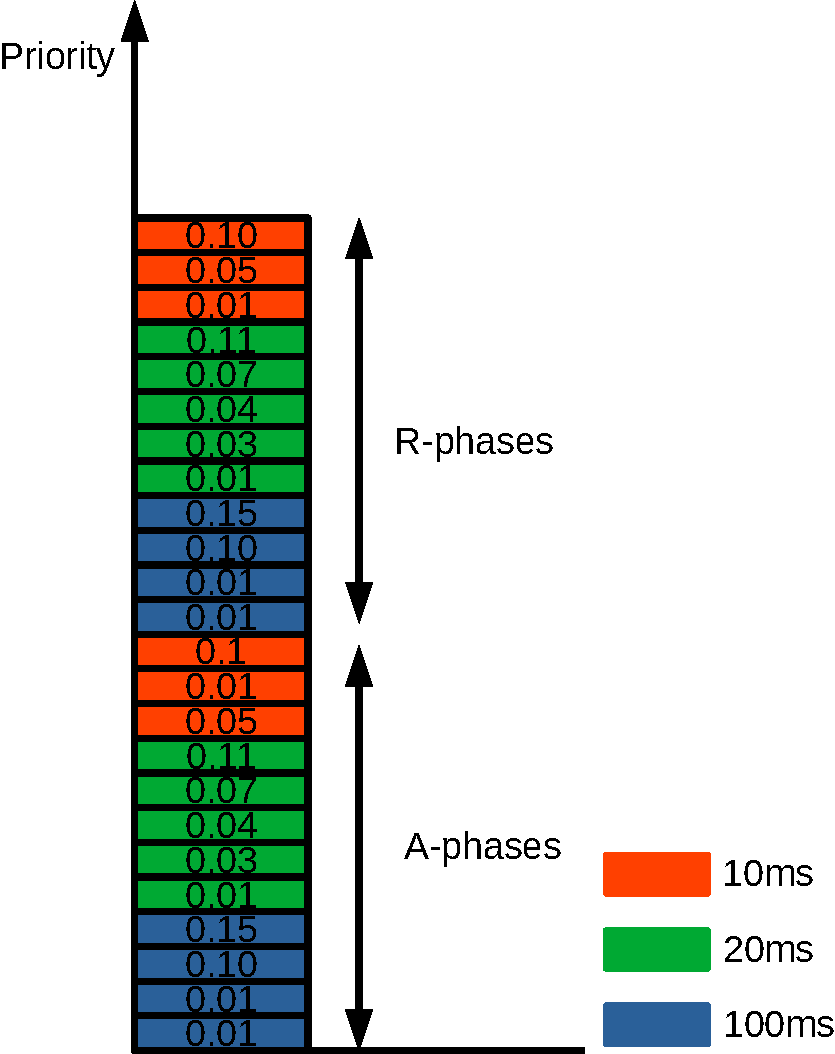
\includegraphics[width=0.8\linewidth]{images/scheduling_priorities.pdf}

    \caption{Priorities assigned according to a HULP scheduler with utilization written on each task}

    \label{fig:scheduling_priorities}

\end{figure}

The general concept of prioritization in this manner is depicted in figure
\ref{fig:scheduling_priorities} which describes how jobs would be prioritized according to
\acrshort{hulp}. The priorities are ordered along the x-axis where higher priorities are higher up
and a job is depicted by a box. It is important to remember that all of the \acrshort{r}-jobs must
have a higher priority than all of the \acrshort{a}-jobs as described in section \ref{sec:iip}. As
can be seen in the figure the highest priority is given to the \acrshort{r}-jobs with the lowest
periods (10ms) colored orange. Within the period the jobs are then prioritized according to their
utilization which is depicted by the number on the job. 


% RMS isn't a good choice as there are many tasks with the same period, and they will just be
% scheduled according to task-id on the task-level


\section{Benchmarking}\label{sec:benchmarking}

To benchmark the \acrshort{aer} \acrshort{iip} job sets have to be generated according to the
\acrshort{aer} model as well as the input restrictions of the \acrshort{np}-test. The input to the
\acrshort{np}-test is in the form of a \acrfull{csv} file. It is a plain-text file where each new
line holds a unique job to be scheduled where the rows columns are separated by commas and represent
the jobs attributes. The columns expected by the analysis tools are as follows.

\begin{itemize}
    \item \textbf{Task ID} - The ID of the belonging task
    \item \textbf{Job ID} - Its unique ID
    \item \textbf{Arrival min} - Its earliest release time
    \item \textbf{Arrival max} - Its latest release time
    \item \textbf{Cost min} - Its \acrshort{wcet}
    \item \textbf{Cost max} - Its \acrshort{bcet}
    \item \textbf{Deadline} - The time at which the job must have finished execution
    \item \textbf{Priority} - Its priority in relation to the other jobs
\end{itemize}



Thus all of the properties of the jobs must be properly generated in order to perform benchmarks.
One option would be to just randomize everything, but this would not be very reflective of any real
systems or applications. Since a lot of the benchmarking will explore how the analysis tool performs
under different utilizations a good starting point would be to explore how tasks sets can be
generated given the total desired utilization and the desired amount of tasks. Generating the
amount of tasks to be constant is important, as tasks sets of different sizes but with the same
utilizations have been shown to have different average schedulability for many schedulers and could
thus have an effect on the results \parencite{sebestyen_simulation-based_2012}. The amount of tasks
generated for a certain utilization should therefor carefully be put into consideration.

Benchmarking of the \acrshort{np}-test is done in three phases. The first phase is the task
generation which generate task sets with a predetermined amount of tasks and a set utilization. This
task set is then passed on to the task transformation phase which transforms the task set into a job
set which follows the \acrshort{aer}-model discussed in section \ref{sec:work_task_model}. The job
set is also on the appropriate form to be used as input for the \acrshort{np}-test which is the
final phase and outputs the result whether the original task set is schedulable or not. The three
phases are depicted in figure \ref{fig:benchmark_toolchain}. The reason for decoupling the three
phases is that any one can be switched out to a counterpart without having to make any changes to
the others as long as the form of the input and output is the same. The remainder of the section
goes into detail of each of the three phases. 

\begin{figure}

    \centering

    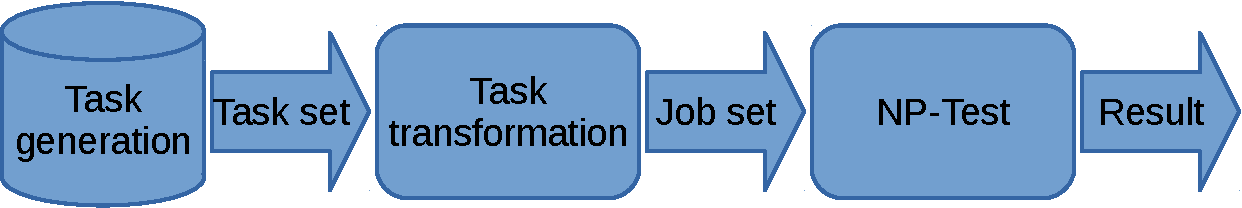
\includegraphics[width=0.8\linewidth]{images/benchmark_toolchain.pdf}

    \caption{Priorities assigned according to a HULP scheduler with utilization written on each task}

    \label{fig:benchmark_toolchain}

\end{figure}


\subsection{Task generation} \label{subsec:task_generation}

The paper \parencite{bini_measuring_2005} goes into great detail explaining some of the common pitfalls
when creating good task sets for benchmarking. It also presents the \textbf{Uunifast} algorithm to
help create fair task sets which is an $O(n)$ algorithm used to create sets of utilization values.
The algorithm takes two inputs, the size of the set to be created (the amount of tasks) and the
total utilization sum of all the tasks. Once the output of the algorithm has been acquired it
becomes a more trivial task to generate task sets by using the given utilizations to create
execution times from periods, or periods from execution times.

After the utilizations have been generated the next step is to create the actual task set. This can
be approached from two different directions. Either the periods of the tasks can be generated, and
from them the execution times using the already generated utilizations. Or the process can be
reversed and the execution times can be generated first and then the periods from them based on the
utilizations. It can be a good idea to create the task set with characteristics of a real
application as it would give valuable information about how the \acrshort{aer} \acrshort{iip} and
the extended \acrshort{aer} model would behave in a real application.

Since the major application of the \acrshort{aer} model lies within the automotive and avionics
sector the task set should cohere to the standards and practices to these industries.  However large
companies tend to be very secretive of their work but luckily there is a standard within the
automotive industry called \acrshort{autosar} that has been agreed upon to make it easier for
cooperation between corporations when developing embedded systems. According to the
\acrshort{autosar} standard, the periods for periodic tasks must be selected from nine predefined
intervals which are 1, 2, 5, 10, 20, 50, 100, 200, 1000 milliseconds. The standard also defines
aperiodic tasks as either being driven by interrupts, or being angle-synchronous, which means that
they are triggered by a certain angle of the crank-shaft, making the period a function of the
rotations-per-minute of the crankshaft. Even though aperiodic tasks are accepted by the analysis
tool they would not contribute significantly to the results of the thesis.

%TODO: Explain the choice to not use the 1000ms period during experiments
Since a set of predefined periods are given the execution times of the tasks can easily be generated
from randomising a period and pairing it with a random utilization from the set created by the
uunifast algorithm. However, the probability distribution for the periods might not be uniform for a
real life system which should be put into consideration when choosing the period. Luckily a research
group at Bosch has released benchmarking data from real world automotive systems to be used for
free by anyone in the paper \parencite{kramer_real_2015}.  The data has been extracted from a
real-world application to a point where it doesn't doesn't give away any \acrfull{ip}-critical
information about the actual application. The actual distribution of the periods from the paper are
given in table \ref{tab:period_distribution}. Since we do not consider angle-synchronous tasks in
this thesis the extra 15\% is simply ignored. In addition, when pairing a 1000ms with any
utilization during benchmarking its \acrshort{a}-phase and \acrshort{r}-phase have a high chance of
having an execution time of above 1ms making it so that no task with a period of 1ms will ever be
schedulable and is thus also ignored. The remaining percentages are scaled such that their
probability sum equals 100\% as shown in the third column in table \ref{tab:period_distribution}.

\begin{table}
    \centering
    \begin{tabular}{| c | c | c |} 
        \hline
        Period & Probability & Adjusted probability  \\
        \hline
        1 ms & 3\% & 5\% \\
        \hline
        2 ms & 2\% & 3\% \\
        \hline
        5 ms & 2\% & 3\% \\
        \hline
        10 ms & 25\% & 29\% \\
        \hline
        20 ms & 25\% & 29\% \\
        \hline
        50 ms & 3\% & 5\% \\
        \hline
        100 ms & 20\% & 24\% \\
        \hline
        200 ms & 1\% & 2\% \\
        \hline
        1000 ms & 4\% & 0\% \\
        \hline
        Angle-synchronous & 15\% & 0\% \\
        \hline
    \end{tabular}
    \caption{Distribution of periods within a real \acrshort{autosar} system. Taken from \parencite{kramer_real_2015}}
    \label{tab:period_distribution}
\end{table}

After pairing a utilization with a period to create the tasks execution time the question remains
how to decide the \acrshort{wcet} and \acrshort{bcet}. Even though the free benchmarks from Bosch
offers a way to generate these from the average execution time and it is accepted by the
\acrshort{np}-test it does not provide much of a benefit to the benchmark. This becomes more clear
in section \ref{sub:task_transformation} but the short reason is that only the \acrshort{wcet} is
used when creating the job set and setting it to something different than what was generated by the
uunifast algorithm will change the total utilization of the task set, which is undesirable.

The execution times of the \acrshort{a}-phase and \acrshort{r}-phase are functions of the size of
the data read and written to the memory during each phase which can be very deterministic if no
cache is assumed and since the phases cant be preempted. The question remains what size to pick
for the phases and it is not trivial. The paper "Scheduling Multi-Rate Real-Time Applications on
Clustered Many-Core Architectures with Memory Constraints"\parencite{becker_scheduling_2018}
contains information about the execution times of the acquisition and restitution phases of 18
different tasks in an engine management system in a car. These could be used to make approximations
of the ratios between the execution times of the three different phases. However, it could be of
interest to benchmark how the schedulability of the job sets is affected by varying the ratios
between the three phases. These ratios are thus instead provided during benchmarking as an input to
the task generator, further explained in section \ref{sec:benchmarking}. The desired values are thus
taken as input to the task generator and are referred to as the \acrshort{a}-ratio and
\acrshort{r}-ratio where each value represents the ratio of the respective phase to the total
utilization of the task.

%The ratios determine how much of the total execution phase, which was determined earlier by the
%utilization and period, should be allocated to the \acrshort{a}-phase and the \acrshort{r}-phase,
%where differing ratios between them is possible. This mean that they "steal" execution time from the
%\acrshort{e} phase. This is in order to not change the total utilization of the task set in any way.

The \acrshort{np}-test accepts the release-time to be defined as an interval in case of release
jitter. This is not used in benchmarking and the worst-case release time is thus defined to be
the same as the best-case release time for all jobs. The priorities of the jobs are then
assigned by a scheduling algorithm discussed in section \ref{sec:scheduling_algorithms}. Even though
creating an even more realistic task set generation is possible the scope could be a thesis topic of
its own and the proposed method is already sufficiently good.

%TODO: Mention that even though one could create a much more accurate task set using the information
%given in free benchmarks it would be hard to adhere it to a set total utilization and it would be
%a large enough scope for a thesis of its own.

\subsection{Task transformation} \label{sub:task_transformation}

As the task generation does not generate job sets which are appropriate as input for the
\acrshort{np}-test they have to be transformed. The transformed job-set can also not hold any
explicit data that would separate it from a regular job-set even though it actually represents tasks
under the \acrshort{aer} model, all this information is instead implicit. This can be done as long
as the task generation phase provides sufficient information about the tasks in its output. The
necessary information, which is provided by the task generation phase, is as follows.

\begin{itemize}
    \item \textbf{Task ID} - The tasks ID
    \item \textbf{Arrival min} - The earliest relative release time
    \item \textbf{Arrival max} - The latest relative release time
    \item \textbf{Computation min} - The \acrshort{bcet} of the execution-phase
    \item \textbf{Computation max} - The \acrshort{wcet} of the execution-phase
    \item \textbf{Acquisition max} - The \acrshort{wcet} of the acquisition-phase
    \item \textbf{Restitution max} - The \acrshort{wcet} of the restitution-phase
    \item \textbf{Deadline} - The relative deadline
    \item \textbf{Priority} - The priority relative to other tasks in the set
    \item \textbf{Period} - The period 
\end{itemize}

So all of this information about a task set is then to be transformed into a job set represented by
the characteristics given in section \ref{sec:benchmarking} as to be accepted as input to the
\acrshort{np}-test. The basic idea in transforming the \acrshort{aer}-modeled task set into a
regular job set is to make the \acrshort{a}-phase and \acrshort{r}-phase of each period into
individual jobs. Although the \acrshort{e}-phase is not turned into its own job it still holds vital
information. The reason is that the jobs are to be scheduled around memory-accesses, and the whole
point of the \acrshort{aer}-model is that the \acrshort{e}-phase holds no memory-accesses to shared
memory and as such doesn't have to directly be taken into account by the scheduler. The way the
execution-phase will be used is to represent the constraint that the interval between the deadline
of the acquisition-phase and the earliest release time of the restitution phase must be that of at
least the \acrshort{wcet} of the execution-phase. This ensure that the acquisition job is not
scheduled until the execution-phase is guaranteed to have finished. 


\begin{algorithm}
    \caption{Task transformation}
    \label{algo:task_transformation}
    \begin{algorithmic}[1]

        
        \renewcommand{\algorithmicrequire}{\textbf{Input:}}
        \Require $W \in [0, 1]$: ratio between A and R windows, $\Gamma$: \acrshort{aer} task set
        

        \State $hyperperiod \gets 0$
        \ForAll{$\tau \in \Gamma$}
            \Comment Find the hyperperiod
            \State $hyperperiod \gets lcm(hyperperiod, \tau_T)$
        \EndFor


        \State $id \gets 1$
        \ForAll{$\tau \in \Gamma$}
            \Comment Create jobs for each task in the task set

            \State $window\_size \gets \tau_{D} - \tau_{r^{min}} - \tau_{C^{max}}$ 

            \For{$i \gets 0, hyperperiod/\tau_T$}
                \State $t \gets i * \tau_T$
                \Comment Absolute time for the period

                \State //Create the acquisition job
                \State $J^{A}_{id} \gets id$
                \State $id \gets id + 1$
                \State $J^{A}_{task\_id} \gets \tau_{id}$
                \State $J^{A}_{r^{min}} \gets t + \tau_{r^{min}}$
                \State $J^{A}_{r^{max}} \gets t + \tau_{r^{max}}$
                \State $J^{A}_{C^{min}} \gets \tau_{acquisition}$
                \State $J^{A}_{C^{max}} \gets \tau_{acquisition}$
                \State $J^{A}_d \gets t + \left \lceil{W * window\_size}\right \rceil $
                
                \State //Create the restitution job
                \State $J^{R}_{id} \gets id$
                \State $id \gets id + 1$
                \State $J^{R}_{task\_id} \gets \tau_{id}$
                \State $J^{R}_{r^{min}} \gets J^{A}_d + \tau_{C^{max}}$
                \State $J^{R}_{r^{max}} \gets J^{A}_d + \tau_{C^{max}}$
                \State $J^{R}_{C^{min}} \gets \tau_{restitution}$
                \State $J^{R}_{C^{max}} \gets \tau_{restitution}$
                \State $J^{R}_d \gets t + \tau_D $

                \State $\mathcal{J} \gets \mathcal{J} \cup \{J^A\} \cup \{J^R\}$
                \Comment Add created jobs to the job set
            \EndFor
        \EndFor
        \State $assign\_priorities(\mathcal{J})$
        \Comment Assigning priorities relies on all jobs having been created

    \end{algorithmic}
\end{algorithm}


The jobs are transformed according to algorithm \ref{algo:task_transformation}. Since a schedule is
bound to repeat itself after one hyperperiod it is sufficient to test the schedulability during this
interval. Thus the algorithm first finds the hyperperiod of the task set by finding the
least-common-multiple of all the periods. It is then sufficient to create the jobs that are released
within the hyperperiod, placing an upper-bound on their release times. This ensures that the
task-transformation will terminate. The jobs are then created from one task at a time until jobs for
all tasks have been created. 

The tasks \textbf{window size} is defined as the total time of the \acrshort{a}-window plus the
\acrshort{r}-window. It is used in conjunction with the window ratio to calculate the actual sizes
of the windows. Since the \acrshort{np}-test requires absolute time (as opposed to relative time
which is relative to the start of the period) the start time for each period is calculated and used
to to transform relative time values to absolute ones. This continues until the hyperperiod is
reached at which no more jobs are created for that task. Since all the jobs are created in pairs of
an \acrshort{a}-job and a \acrshort{r}-job where the \acrshort{a}-job is created first and given an odd
job-id as required and further explained in section \ref{sec:scheduling_algorithms}. Its release
time is then transformed from the tasks relative release time to an absolute release time. Its
worst-case execution time is then assigned according to the execution time of the \acrshort{a}-phase
in the task. The deadline is then calculated from the window size and the window ratio which is
given as input to the algorithm and transformed to an absolute time. The \acrshort{r}-phase is then
created in a similar manner, but given an even job-id. Its release times are calculated as the
deadline of the \acrshort{a}-job plus the \acrshort{wcet} of the \acrshort{e}-phase. The
\acrshort{r}-job gets its execution time from the execution time of the \acrshort{r}-phase in the
task. The deadline is then assigned according to the tasks deadline, but transformed into absolute
time. When all the jobs for every task have been created they are all assigned priorities according
to the one of the scheduling algorithms described in section \ref{sec:scheduling_algorithms}. This
is because the priorities describe a relation between the jobs, thus all the jobs must sometimes be
created before the priorities can be assigned. 


\subsection{Running benchmarks}\label{subsec:running_benchmarks}

As part of benchmarking a set of experiments will be ran to test what effect different input
variables will have on the schedulability ratio. Each variable that will be put into consideration
is shortly described in the rest of this section.

The experiments will be running on a "HP Z210 Workstation" with a quad-core Intel Core i7-2600 CPU
\@3.40GHz and 16 GiB of memory.

The idea of benchmarking is to first recognise the dependent and independent variables of the system
and then make changes to the independent variables and see what effect they have on the dependent
variables. The dependent variable of most interest is the \textbf{schedulability ratio} which is the
ratio between schedulable task sets and the total amount of task sets tested. The independent
variables are explained in the following list.

\begin{itemize}

    \item \textbf{Task amount} - The total amount of tasks to be scheduled
    \item \textbf{Core amount} - The amount of cores available for jobs to be scheduled onto.
    \item \textbf{Scheduling algorithm} - The algorithm used to schedule the system. 
    \item \textbf{\acrshort{a}-ratio} - The execution time of the \acrshort{a}-phase as a ratio of
        the tasks utilization.
    \item \textbf{\acrshort{r}-ratio} - The execution time of the \acrshort{r}-phase as a ratio of
        the tasks utilization.
    \item \textbf{Window ratio} - The ratio between the \acrshort{a}-window and \acrshort{r}-window.
    \item \textbf{Utilization} - The total utilization of all tasks summed.

\end{itemize}

%TODO: Explain why the input is chosen the way it will be, 10% a and r cycles, the task amount, the
%core amount etc.

The following sections describe each experiment that tests a different independent variable and
what the static values for the untested independent variables are set to. When generating the task
sets the random number generator is seeded with the same number to ensure the same task sets are
used for different experiments and graphs to increase the reliability of the experiments. 

\subsubsection{Task amount}

The idea is to use task amount as a variable and see how the schedulability ratio changes as an
effect on how many tasks need to be scheduled when the other variables are constant. Smaller amount
of tasks leads to larger execution times of each task and vise versa and should therefor have an
effect on the utilization. The experiment will test task sets of size 1 to 1000 with size 100
increments. It will also test task sets of size 1 to 150 with size 2 increments for better
resolution for smaller task sets. The \acrshort{a}-ratio and \acrshort{r}-ratio will be set to 0.1,
the window-ratio will be set to 0.6, the utilization will be set to 0.5 for both experiments. To
make sure that memory accesses is the bottleneck the core amount is set to be larger than the amount
of tasks, such that in worst case each task has its own dedicated core. The used scheduling
algorithm will be \acrshort{edf} and the experiment will be iterated 100 times for each data point
for both intervals of task sizes to create the schedulability ratio. Since the runtime rises rapidly
with the size of the task set the iterations are set to a lower amount than for some of the other
experiments.


\subsubsection{Core amount}

As the other experiments bottleneck the memory accesses by using more cores than tasks it should
also be tested what the effects are when the amount of cores are a possible bottleneck. This will be
done by constraining the amount of cores that are available for tasks to be scheduled onto them. The
size of the task set is chosen to 10 tasks and as such the core amount will be varied from 10 down
to a single core. In addition to cores being varied the utilization of the task sets will also be
varied starting from 0.1 and incremented up to 4.0 with a step size of 0.1. The \acrshort{a}-ratio
and \acrshort{r}-ratio are both set to 0.1 and the window-ratio is set to 0.6. The scheduling
algorithm used will be \acrshort{edf}. Each step in utilization will be iterated 100 times to create
a reliable average schedulability ratio.


\subsubsection{Window ratio}

The window ratio describes the ratio of the size difference between the \acrshort{a}-window and
\acrshort{r}-window as the two phases doesn't necessarily have to be given the same amount of time
to complete execution. So this will examine what characteristics the system exhibits for different
sizes of the windows. Since this can vary greatly depending on the utilization it should also be
varied. For the window sizes nine different sizes while be tried ranging from 10\% to 90\% of the
total size allocated to the \acrshort{a}-window, where all of the remaining percentages are
allocated to the \acrshort{r}-phase. The utilization will range from 0 to 4 with an increment size
of 0.1, each step iterated 1000 times to create a schedulability ratio. The task amount is set to
15, the The scheduling algorithm used is \acrshort{edf} and the core amount is set to be larger than
the task amount to bottleneck the memory. The \acrshort{a}-ratio and \acrshort{r}-ratio is both set
to 0.1.

\subsubsection{Scheduling algorithms}

The different scheduling algorithms that will be tested have been explained in section
\ref{sec:scheduling_algorithms}. Each algorithm will be tested for different utilizations ranging
from 0 to 4.2 with increments of 0.1. Each incrementation in utilization is iterated 1000 times to
create a schedulability ratio for that utilization. The \acrshort{a}-ratio and \acrshort{r}-ratio
are both chosen to 0.1 and the window ratio is set to 0.5. The task amount is set to 15 and the
cores are set to be larger as to bottleneck the memory and not the cores.


\chapter{Results} \label{ch:result}

This chapter shows the results from the benchmarking of the analysis tool explained in section
\ref{subsec:running_benchmarks}. Section \ref{sec:result_window_ratios} show the resulting
schedulability ratio from testing a variety of window ratios for the \acrshort{aer}-tasks, section
\ref{sec:task_amount} shows the schedulability ratio when varying the amount of tasks in the task
set, section \ref{sec:results_core_amount} shows the schedulability ratio when differing the amount of cores
available in the system and section \ref{sec:results_scheduling_algorithms} shows the schedulability
ratio for different tested scheduling algorithms when varying the utilization of the task set.

\section{Window ratios}\label{sec:result_window_ratios}

\begin{figure}[H]

    \centering

    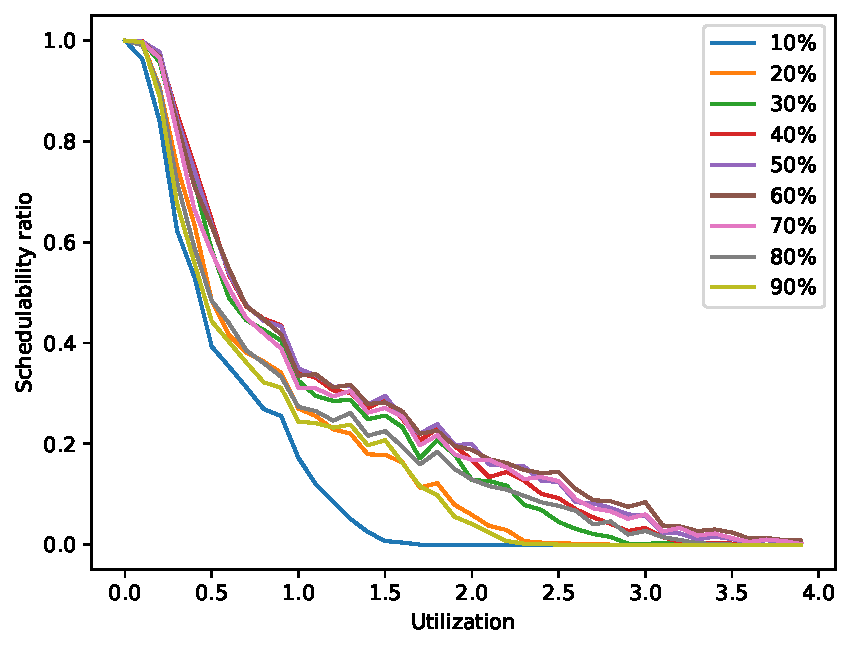
\includegraphics[width=1.0\linewidth]{images/window_ratio.pdf}

    \caption{The schedulability ratio of different window ratios as an effect of the total
        utilization of the task set.}

    \label{fig:window_ratio}

\end{figure}

All of the window ratios have a quick initial fall of in schedulability before it planes out to a
slower decent as shown in figure \ref{fig:window_ratio}. Most of the lines stay clumped together
throughout except for 10\% which takes on a faster decline than the others. The lines for 90\% and
20\% are close to each other throughout and fall a bit below the majority of the lines when
approaching a higher utilization. Towards higher utilizations the 60\% window ratio seems to perform
better than all others, but during lower utilizations although it being amongst the top ones it is
sometimes surpassed by both the 50\% and 40\% window ratios.


\begin{figure}[H]

    \centering

    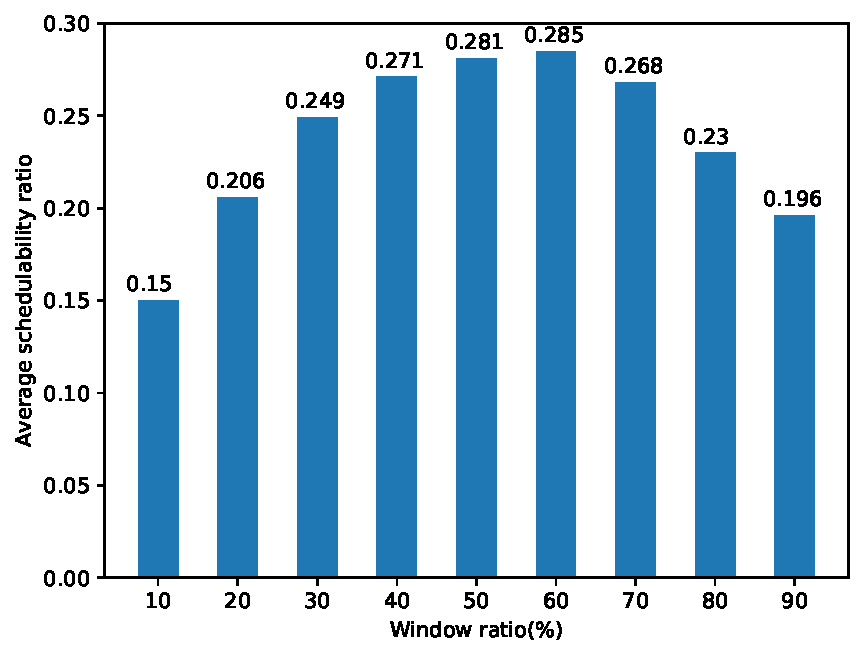
\includegraphics[width=1.0\linewidth]{images/window_ratio_averages.pdf}

    \caption{Priorities assigned according to a HULP scheduler with utilization written on each task}

    \label{fig:window_ratio_averages}

\end{figure}

Averaging the schedulability ratio for all tested utilizations for every window ratio shows that a
window ratio of 60\% has the highest average schedulability ratio overall in figure
\ref{fig:window_ratio_averages}. Furthermore, choosing a window ratio that gives more time to the
\acrshort{r}-phase (high window ratio) seems to favor the average schedulability ratio compared to
given the same size of the window to the \acrshort{a}-phase.

\section{Task amount} \label{sec:task_amount}

\begin{figure}[H]

    \centering

    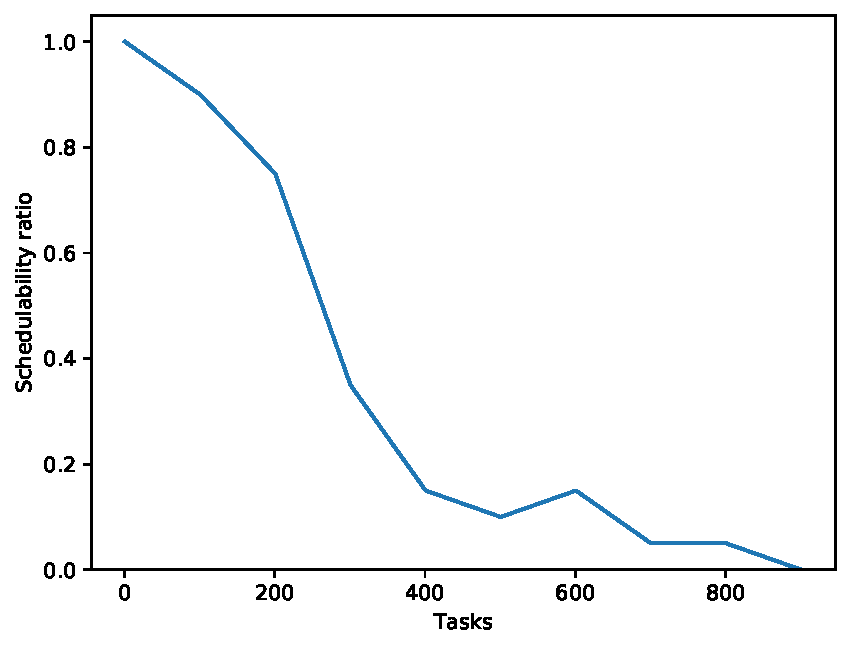
\includegraphics[width=1.0\linewidth]{images/task_amount_2.pdf}

    \caption{Priorities assigned according to a HULP scheduler with utilization written on each task}

    \label{fig:task_amount_2}

\end{figure}

When looking at the task amount from a macro-level as in figure \ref{fig:task_amount_2} it is shown
that the schedulability ratio has a steady decline as more tasks are added to the task set. It was
unable to schedule any task sets at all as the sizes approached 1000 tasks. However, when looking at
the schedulability ratio at a micro-level between 0 and 250 tasks as shown in figure
\ref{fig:task_amount_1} there is a clear difference. There is a quick fall-of in the schedulability
ratio for task sets of low sizes, but it then halts and the schedulability ratio is then improved
again and peaking somewhere around a task set size of 100 to 175 tasks before once again falling of,
at a much slower tempo.

\begin{figure}[H]

    \centering

    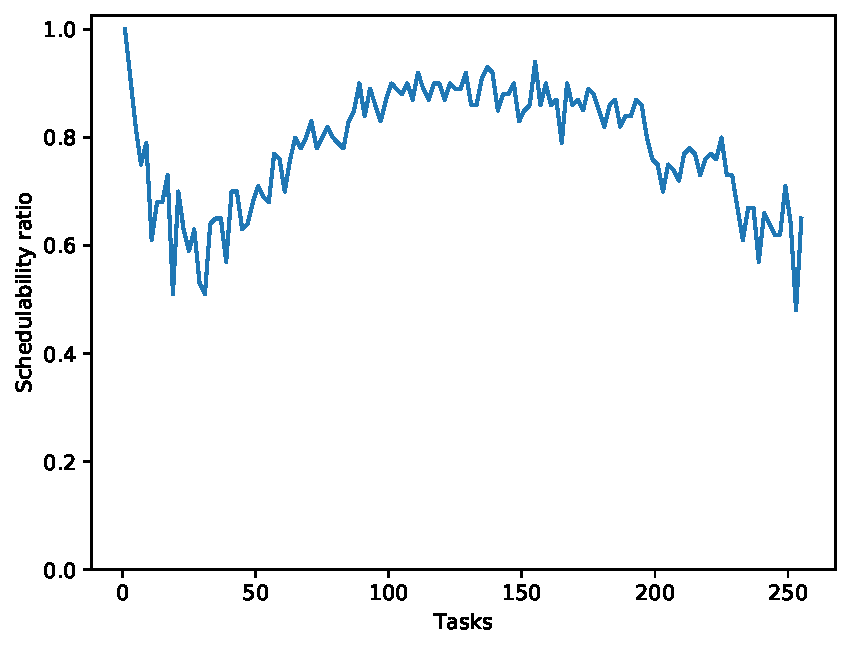
\includegraphics[width=1.0\linewidth]{images/task_amount_1.pdf}

    \caption{Priorities assigned according to a HULP scheduler with utilization written on each task}

    \label{fig:task_amount_1}

\end{figure}


\section{Core amount}\label{sec:results_core_amount}

\begin{figure}[H]

    \centering

    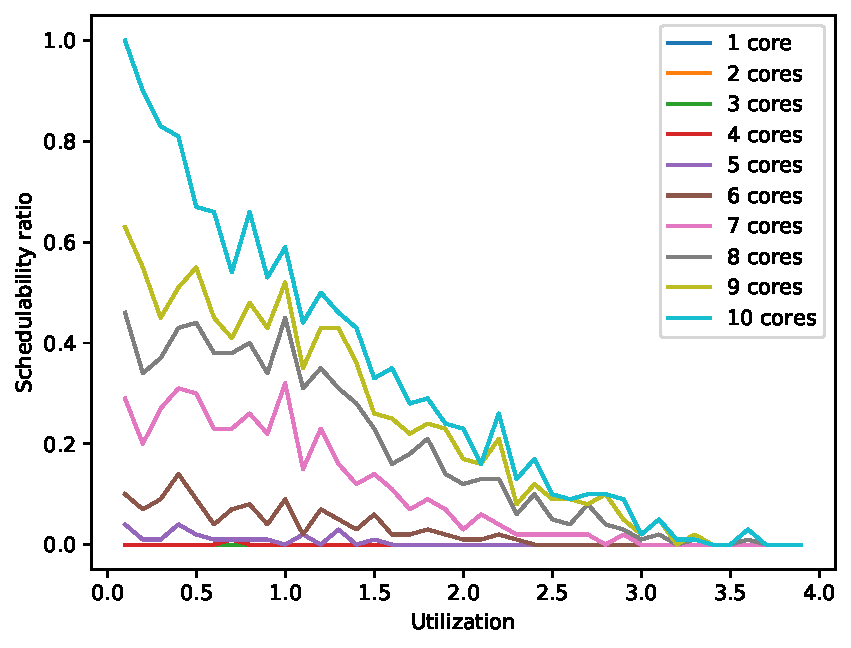
\includegraphics[width=1.0\linewidth]{images/core_amounts.pdf}

    \caption{Priorities assigned according to a HULP scheduler with utilization written on each task}

    \label{fig:core_amounts}

\end{figure}

The first thing to notice is that a core amount of 4 and below are unable to schedule any task sets
at all, even for a utilization of 0.1. Furthermore it is very clear that the core amount have a
large impact on the schedulability ratio. Reducing the core amount down from 10 to 9 reduces the
schedulability ratio by almost 0.4 as seen in figure \ref{fig:core_amounts}. Each reduction in the
amount of cores then substantially lowers the schedulability ratio for a utilization of 0.1 down
until the schedulability ratio hits 0 for 4 cores. Figure \ref{fig:core_amounts_averages} also shows
the steady decline in schedulability ratio as the amount of cores are decreased.

\begin{figure}[H]

    \centering

    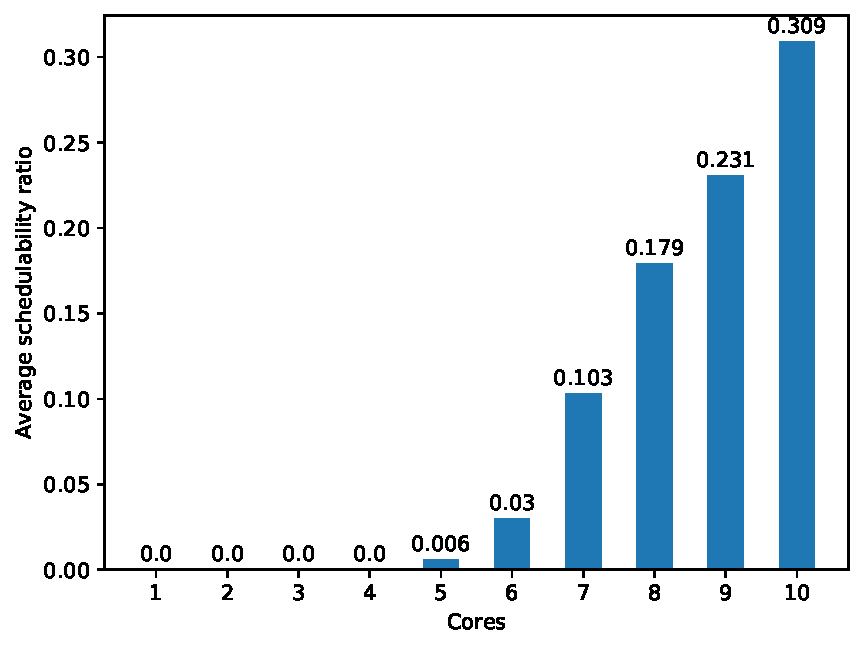
\includegraphics[width=1.0\linewidth]{images/core_amounts_averages.pdf}

    \caption{Priorities assigned according to a HULP scheduler with utilization written on each task}

    \label{fig:core_amounts_averages}

\end{figure}

\section{Scheduling algorithms} \label{sec:results_scheduling_algorithms}

\begin{figure}[H]

    \centering

    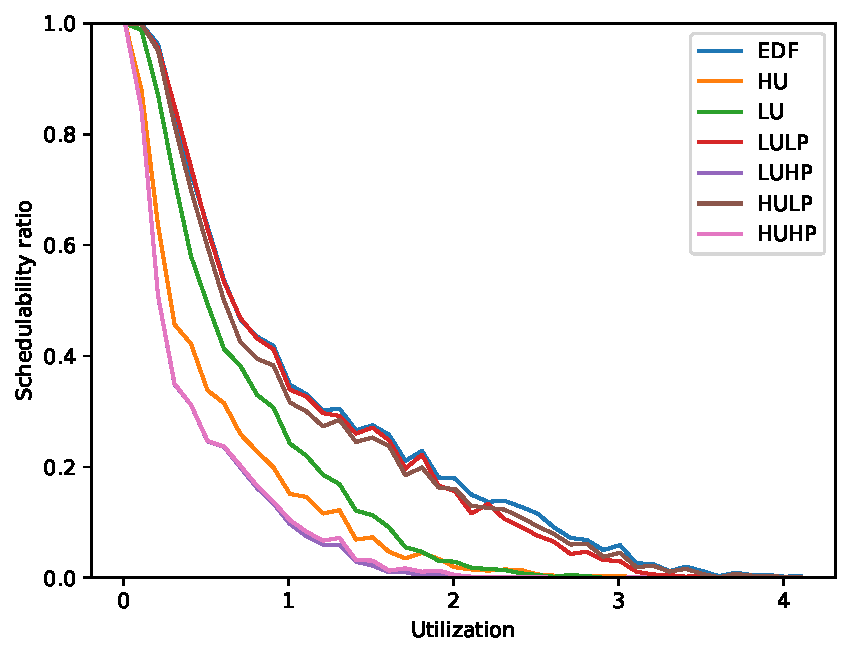
\includegraphics[width=1.0\linewidth]{images/sched_algos.pdf}

    \caption{Priorities assigned according to a HULP scheduler with utilization written on each task}

    \label{fig:sched_algos}

\end{figure}

The worst scheduling algorithms are shown to be the \acrshort{huhp} and \acrshort{luhp} while the
best ones were \acrshort{edf}, \acrshort{hulp} and \acrshort{lulp} as can be seen in figure
\ref{fig:sched_algos}. All of the algorithms had a quick initial drop off in schedulability ratio
when increasing the utilization from 0 towards 1.0. The drop in schedulability ratio then takes on a
slower decent, especially slow for \acrshort{edf}, \acrshort{lulp} and \acrshort{hulp} which keeps
the highest schedulability ratios until they approach schedulability ratio of 0. The \acrshort{huhp}
and \acrshort{luhp} quickly decent to a schedulability ratio of 0 at around a utilization of 2, far
before any of the other algorithms. In between the top and bottom performers are \acrshort{lu} and
\acrshort{hu} which out of \acrshort{lu} performs better for lower utilizations up until right
before a utilization of 2 where they then continue to perform equally bad.

As can be seen from figure \ref{fig:sched_algos_averages}, which represents the average
schedulability ratio of all utilization points tested for each of the scheduling algorithms, the top
performers are as mentioned earlier \acrshort{edf}, \acrshort{lulp} and \acrshort{hulp} with
\acrshort{edf} in the absolute top. The worst performers are once again shown to be \acrshort{luhp}
and \acrshort{huhp} and \acrshort{hu} and \acrshort{lu} being middle performers with \acrshort{lu}
on top.

\begin{figure}[H]

    \centering

    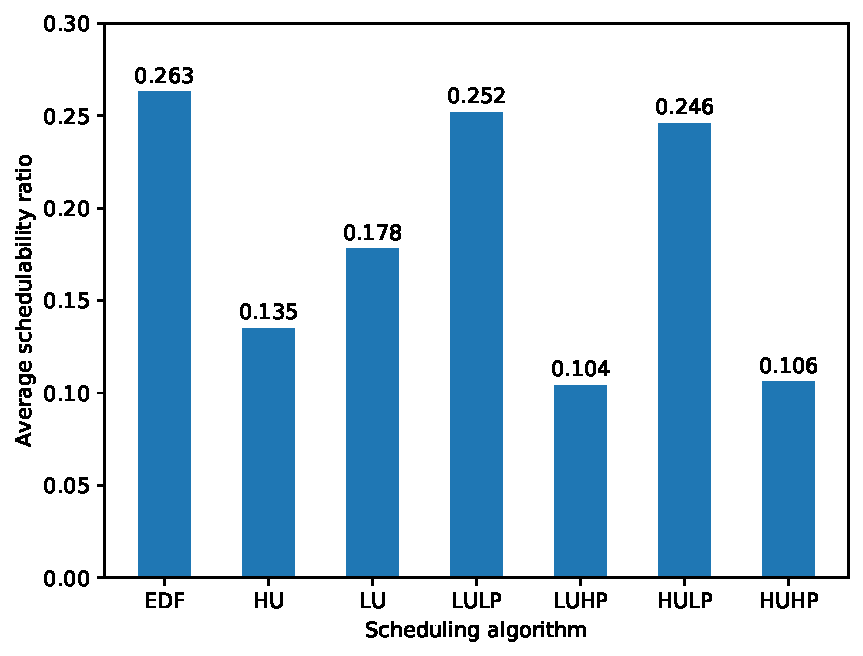
\includegraphics[width=1.0\linewidth]{images/sched_algos_averages.pdf}

    \caption{Priorities assigned according to a HULP scheduler with utilization written on each task}

    \label{fig:sched_algos_averages}

\end{figure}

\chapter{Discussion} \label{ch:discussion}

% Window ratios
As discussed in section \ref{sec:result_window_ratios} giving more time to the \acrshort{a}-phase
rather than the \acrshort{r}-phase favors schedulability ratios. This is probably due to how the
scheduling algorithms are designed to always give all of the \acrshort{r}-phase jobs a higher
priority than the highest priority \acrshort{a}-phase job. This has the effect that whenever an
\acrshort{a}-job and an \acrshort{r}-job are both available the \acrshort{r}-job will always be
scheduled first. Thus the \acrshort{a}-job will be pushed closer to its deadline, decreasing its
slack time and also increasing the chance that it will miss its deadline. So if the
\acrshort{r}-jobs on average will have a larger slack time than the \acrshort{a}-jobs, some of the
slack time that \acrshort{r}-jobs have can instead be reassigned to the \acrshort{a}-jobs to
increase their slack times resulting in fewer deadlines missed and a higher schedulability ratio. As
is shown from the results the optimal window-ratio is to allocate, out of the tried window ratios,
60\% of the time to the \acrshort{a}-job. Even though this thesis assumes a very deterministic
execution time for the \acrshort{e}-phase, a drawback of the model when relaxing this assumption is
the naive use of \acrshort{wcet} as the gap between the \acrshort{a}-window and \acrshort{r}-window.
In a real application the \acrshort{wcet} can be many orders of magnitudes larger than the
average-case, which means that the \acrshort{a}-window and \acrshort{r}-window would be
significantly smaller than what is necessary for the average case, thus decreasing schedulability.
This can be improved upon by further extension of the task model which is discussed in section
\ref{sec:future_work}.

% Task amount

As seen in figure \ref{fig:task_amount_1} there is a sweet spot of task set sizes where the
schedulability ratio is at a local maximum. There is also problem area for small task sets where the
schedulability ratio quickly drops-off to then recover. The initial drop-off in schedulability ratio
for task sets of small sizes are probably due to each task getting a higher execution time. This
increases the risk that a task with a high period gets a high execution time, which in turn can
make the execution time of the tasks \acrshort{a}-phase or \acrshort{r}-phase to be as high,
or higher than the period of low-period tasks. This would then increase the low-period tasks chance
to miss their deadline as they might get blocked for accessing the memory through their whole period
by a single high-period task. As the task set size increases the execution times of each individual
task also decreases on average, which decreases the risk of any low-period tasks missing their
deadline. This problem was hypothesised and explained in section \ref{subsec:task_generation} which
resulted in periods of 1000ms being removed from any generated task set. The schedulability ratio
within this problem area could probably be increased further by shrinking the interval between the
lowest-period and the highest-period of all tasks the task sets by, for example, also removing
periods of 100ms and 200ms. The schedulability ratio would also expect to improve for the other
experiments, as these typically had a task set of sizes within the problem area.

% Scheduling algorithms

When looking at the different tried scheduling algorithms it is evident that \acrshort{edf} is the
top performing algorithm. Seeing that \acrshort{huhp} and \acrshort{luhp} both have the lowest
average schedulability ratio of all the algorithms and \acrshort{hulp} and \acrshort{lulp} had the
highest average schedulability ratios after \acrshort{edf} it seems that prioritising jobs with a
low priority boosts schedulability immensely. Jobs with a lower period are more probable to have its
deadline closer than a higher period job for job sets where the period equals its relative deadline.
Therefor, putting a higher priority on the jobs with a lower period should decrease missed deadlines
and increase schedulability, which is indeed reflected in the results as can be seen in figure
\ref{fig:sched_algos}. This is also the theory which the scheduling algorithm \acrshort{rms}
originates from. And as discussed in section \ref{sec:scheduling_algorithms} the four algorithms
which take period into account from the ones tested were an extension of the \acrshort{rms}
algorithm. 

The results also show that prioritising jobs within their periods according to their utilization
does not have a significant impact on schedulability. This could be due to the low amount of tasks
in the task set. A task set of size 15 means that the amount of tasks with the most common periods
(10ms or 20ms with a distribution of 29\% of tasks, see table \ref{tab:period_distribution}) is on
average only 4.35 tasks. The \acrshort{a}-jobs for the tasks of same periods will have different
deadlines depending on how large the \acrshort{e}-phase of the same task is. A larger
\acrshort{e}-phase means that both the \acrshort{a}-phase and \acrshort{r}-phase will have shorter
time to execute as it will effectively shrink their windows within which they are able to be
scheduled.

When looking at the results of reducing the amount of cores to be less than the amount of tasks in
the task set, presented in section \ref{sec:results_core_amount}, it is evident that it has a large
detrimental effect on the schedulability ratio. Even though this is to be expected to some degree it
is most likely exaggerated due to the nature of the extended \acrshort{aer} task model (explained in
section \ref{sec:work_task_model}). A big drawback of the model is that whenever the amount of tasks
that share any period exceeds the amount of cores in the system it will never be schedulable no
matter its total utilization. And having just several tasks with the same period is probably
detrimental to the schedulability ratio. This can be demonstrated by imagining a task set of 3 tasks
that are to be scheduled onto two different cores. The tasks all have the same period of 100ms,
\acrshort{e}-phase (\acrshort{wcet}) of 2ms, \acrshort{a}-phase of 1ms and \acrshort{r}-phase of 1ms
and a window ratio of 50\%. This makes the \acrshort{a}-window cover the first 49ms of the
scheduling window and the \acrshort{r}-window cover the last 49ms of the scheduling window. The
middle 2ms is covered by the \acrshort{e}-phase (\acrshort{wcet}). Two of the tasks are instantly
scheduled onto the two available processors while the third task is left idle. After 1ms both of the
scheduled tasks \acrshort{a}-phases will have finished and their \acrshort{e}-phases can start and
will finish 2ms later. At this point both of the processors will become idle, but the third idle task
cannot be scheduled onto either of them as their \acrshort{r}-phases are yet to finish. These will
however not be release until 51ms after the release time of the \acrshort{a}-phases of all three
tasks. At this point the deadline of the \acrshort{a}-phase of the idle task will already have
passed and the deadline is missed.

Not only is it a problem that the task sets with more tasks of a single period than the amount of
cores is unschedulable but also as described that the cores are idle a long time when the
\acrshort{a}-phase is scheduled early inside the \acrshort{a}-window and cant be utilized. This is
also true for when the \acrshort{r}-jobs are scheduled late in their \acrshort{r}-window. The
worst-case scenario being that the \acrshort{a}-job is scheduled just as its released and the
\acrshort{r}-job is scheduled as close to its deadline as possible. This would leave the occupied
core idle without being able to do any actual work for what might be a long time. This does not
matter when the amount of tasks are the same or smaller than the amount of cores, but should be
expected to become a larger problem when the task set grows or the amount of cores are lowered
making them the bottleneck instead of the memory.

It is important to realize that the utilization of the task set does not reflect the utilization of
the memory. In all of the experiments presented in chapter \ref{ch:result} an \acrshort{a}-ratio and
\acrshort{r}-ratio of 0.1 was used. This means that out of the total utilization of a job 10\% of it
comes from the \acrshort{a}-phase, 80\% from the \acrshort{e}-phase and the remaining 10\% from the
\acrshort{r}-phase. When taking all of this into account the utilization of the memory will just be
the \acrshort{a}-phases and \acrshort{r}-phases which together accounts for 20\% of the total
utilization. So in the results, chapter \label{ch:results}, when the utilization totals for
example 1.0 this is the total utilization of all the cores. The utilization of the memory will then
be 20\% of this equalling a utilization of 0.2.

As discussed in section \ref{subsec:running_benchmarks} there are a lot of different independent
variables that all affect the schedulability ratio. Even tough a lot of different values are tried
for the different variables to show their general affect on the schedulability ratio it is a very
complex system and different combinations of values are not tried very extensively in this thesis.
Different results could  have been reached for other combinations of values for the
variables and also for different ways of generating tasks, but the general effect that changing each
of the independent variable has on the schedulability ratio would most likely be the same which is
of interest. 

% Discuss the utilization only being 20% of what is actually shown

% A better thing would be to order jobs according to EDF inside of periods
%   - Actually prio according to LPHU should mirror EDF (inside periods), as the highest utilization
%   tasks will also have the earliest deadlines for the A-jobs.
%       - Not true for R-jobs, hard to draw any conclusions about them, priorities should be same as
%       least-slacktime first

% Using WCET for the E-phase is very naive

% Prio should not matter for R-jobs, they are either schedulable or they are not

% Probably only the lowest-prio job within a period matters, because thats the one who misses its
% deadlin. 


% EDF outperforms all others
% Low period seems to be second best, utilization doesn't matter that much when period is taken into account

% Describe how the task model requires that there are not more number of tasks of a given period
% than the total amount of cores in the system, as it will lead to the schedule being not feasible.

% Complex system, many different dependent variables that can be changed

% Task model in combination with the task periods are probably a poor combination

% A-jobs that are scheduled early in the window and R-jobs scheduled late in their window creates a
% huge gap were the processors is idle.

\section{Conclusions}

The \acrshort{aer}-task-model has been extended such that it can be used with the state-of-the-art
timing analysis tool known as the \acrshort{np}-test. Using the \acrshort{aer}-model has earlier
been shown to improve the schedulability ratio of task sets using a memory-centric schedulability
approach instead of a usual core-centric approach used by most multi-core schedulers. This reduces
the problem to a single-core problem where jobs memory accesses are scheduled (there is only one job
accessing the memory at a time) which allows for an existing schedulability analysis tool to be
used. A new \acrshort{aer} \acrshort{iip} is also developed that is used by the analysis tool for it
to be useful together with the extended task model. The \acrshort{aer} \acrshort{iip} successfully
makes sure that no new job can be scheduled while there are no free cores for the job to be
scheduled onto and enables task sets under the extended \acrshort{aer} model to have their
schedulability analyzed. 

Different values are tried for the independent variables in the task sets used as input to the
schedulability analysis tool to check their effect on the schedulability ratio. The results show
that \acrshort{edf} outperforms all other tested schedulers, and for this a window ratio of 60\% was
also optimal. There is also a sweet spot in schedulability ratio when the task set contains
somewhere between 100 to 150 tasks, but 0 to ~300 tasks is fine without decreasing the
schedulability ratio too much. The task model performs the best when the amount of cores exceed the
amount of tasks, which is not realistic in all cases, but the performance is quickly decreased when
the amount of cores are decreased below the amount of tasks.

% Task model has been created that can be used in conjunction with an exact schedulability analysis
% tool


% EDF is best algorithm, 60% is best window ratio, 100-150 tasks is optimal, but anywhere between 0-
% ~300 is fine. Cores should ideally be larger than the amount of tasks while running in an autosar
% system.

% How good is it actually? Maybe add this to discussion



\subsection{Future work}\label{sec:future_work}

Since the developed task-model puts heavy constraints on when the \acrshort{a}-jobs and
\acrshort{r}-jobs can be scheduled by creating windows for them within which they are to be
scheduled it would be of interest to soften this constraint as it can be expected to increase the
schedulability ratio. The reason for the constraint is for the \acrshort{a}-phase to always execute
before the \acrshort{e}-phase and \acrshort{r}-phase as well as the \acrshort{e}-phase to always
execute before the \acrshort{r}-phase starts. This describes precedence constraints in how the jobs
are scheduled, and is something that the analysis tool already is able to deal with. The task model,
however, requires a special type of precedence. The \acrshort{e}-phases are not explicitly scheduled
by the scheduler as they have nothing to do with the memory, but they are still required to finish
execution before the \acrshort{r}-phase is allowed to begin. An idea then could be to pose a special
type of precedence constraint where a \acrshort{r}-job must not only wait for its \acrshort{a}-job
to finish, but must also wait x amount of time after the \acrshort{a}-job has finished before the
\acrshort{r}-job is allowed to start execution. Time x would then be represented by the
\acrshort{wcet} of the \acrshort{e}-phase similarly to how the task model produced in the thesis
works. 

The limitation that the amount of tasks with the same period cant be larger than the amount of cores
in the system has been discussed. This is an effect of the \acrshort{e}-phase of each task being
placed at the same point in time for each task. It could thus be of interest to see what effect
moving the \acrshort{e}-phase around within the schedulability window (i.e. changing the tasks
window-ratio) to be different for each individual task within the same period. It would be expected
to have an effect on the schedulability ratio as it should, under the right circumstances, allow for
more tasks with the same period than the amount of cores to be schedulable.

The model can further be extended to make it more accurately represent reality. Release jitter can be
added to the tasks by adding it to the \acrshort{a}-job, the naive way of using the \acrshort{wcet}
of the \acrshort{e}-job to model the time-interval required from the latest possible completion of
the \acrshort{a}-job to the earliest possible scheduling of the \acrshort{r}-job can be improved
upon by modelling the \acrshort{wcet} and \acrshort{bcet} of the \acrshort{e}-job as release jitter
for the \acrshort{r}-job. The deadline of the \acrshort{a}-job plus the \acrshort{bcet} of the
\acrshort{e}-job is the earliest possible starting time of the \acrshort{r}-job and the deadline of
the \acrshort{a}-job plus the \acrshort{wcet} of the \acrshort{e}-job is the latest time at which
the \acrshort{r}-job will be available for scheduling. This time interval can simply be modeled as
the release jitter for the \acrshort{r}-job. Furthermore, relaxing the assumption that the
\acrshort{a}-jobs and \acrshort{r}-jobs are always constant in time is possible by modelling them
with a \acrshort{wcet} and \acrshort{bcet} of their own. All of these proposals are already
implemented in the \acrshort{np}-test and only requires an extension of the task model.


% Print the bibliography (and make it appear in the table of contents)
\printbibliography[heading=bibintoc] 

% Start the appendix section
\appendix


\end{document}
